% PLANTILLA APA7
% Creado por: Isaac Palma Medina
% Última actualización: 25/07/2021
% @COPYLEFT

% Fuentes consultadas (todos los derechos reservados):  
% Normas APA. (2019). Guía Normas APA. https://normas-apa.org/wp-content/uploads/Guia-Normas-APA-7ma-edicion.pdf
% Tecnológico de Costa Rica [Richmond]. (2020, 16 abril). LaTeX desde cero con Overleaf (1 de 3) [Vídeo]. YouTube. https://www.youtube.com/watch?v=kM1KvHVuaTY Weiss, D. (2021). 
% Formatting documents in APA style (7th Edition) with the apa7 LATEX class. https://ctan.math.washington.edu/tex-archive/macros/latex/contrib/apa7/apa7.pdf @COPYLEFT

\documentclass[stu,12pt,letterpaper,donotrepeattitle,floatsintext,natbib]{apa7}

% Preámbulo
% preamble.tex - paquetes y configuraciones comunes
\usepackage[utf8]{inputenc}
\usepackage[T1]{fontenc}
\usepackage{lmodern}
\usepackage[spanish]{babel}
\usepackage{graphicx}
\usepackage{float}
\usepackage{placeins}
\usepackage{microtype}
\usepackage{booktabs}
\usepackage{hyperref}
\usepackage{csquotes}
\usepackage{amsmath,amssymb}
\usepackage[normalem]{ulem}
\usepackage{caption}
\usepackage{subcaption}

% Comandos personalizados
\newcommand{\HRule}{\rule{\linewidth}{0.5mm}}

% Definición útil heredada del template: un párrafo con título y salto de línea
\newcommand{\myparagraph}[1]{\paragraph{#1}\mbox{}\\}


% Portada
\title{\Large Desarrollo de una aplicación educativa 3D para la gamificación de tareas en contextos educativos secundarios, institucionales y universitarios}
\author{Fernando Marcos Chocce Janampa \\ Abel Mauricio Santisteban Gamboa}
\authorsaffiliations{INSTITUTO SUPERIOR TECNOLÓGICO TECSUP - DEPARTAMENTO DE TECNOLOGÍA DIGITAL}
\course{Diseño y desarrollo de software: Proyecto de fin de carrera}
\professor{Elliot Garamendi - Jaime Gómez}
\duedate{Lima - Perú, 2025}

\begin{document}
\maketitle

% Índices
\pagenumbering{roman}
\renewcommand\contentsname{\largeÍndice}
\tableofcontents
\setcounter{tocdepth}{2}
\newpage
\renewcommand{\listfigurename}{\largeÍndice de fíguras}
\listoffigures
\newpage
\renewcommand{\listtablename}{\largeÍndice de tablas}
\listoftables
\newpage
\pagenumbering{arabic}

% Incluir capítulos
\section{RESUMEN}

El presente proyecto surge como respuesta al desalineamiento existente entre las tareas educativas y la motivación de los estudiantes en contextos secundarios, institucionales y universitarios. En el sistema educativo actual, los profesores asignan tareas de investigación que muchos estudiantes perciben como poco útiles para su vida real, lo que provoca que prioricen aprobar antes que aprender genuinamente \cite{deci2017}. Ante esta percepción de irrelevancia, los alumnos recurren a atajos digitales como copiar contenido de internet, transcribir sin analizar, o usar herramientas de inteligencia artificial que proporcionan respuestas inmediatas sin fomentar el proceso crítico \cite{chen2023}. Esta problemática genera un aprendizaje superficial donde las tareas se cumplen sin una comprensión real del contenido, desaprovechando el potencial educativo de las herramientas tecnológicas disponibles \cite{martinez2023}.

Se propone una aplicación educativa 3D para la gamificación de tareas. La solución consiste en una aplicación para docentes y estudiantes, donde acceden a un mundo virtual medieval gamificando las actividades académicas en misiones y aventuras. Este ecosistema educativo digital automatiza el ciclo de enseñanza-aprendizaje desde la creación de contenidos hasta la evaluación y seguimiento del progreso de cada estudiante.

El desarrollo implementará componentes como autenticación segura, entornos 3D virtuales inmersivos, sistemas de misiones y recompensas, evaluación integrada y análisis de progreso. La plataforma incorporará tecnologías de inteligencia artificial para personalización del aprendizaje. Adicionalmente, se integrará con plataformas educativas existentes como Canvas, Discord y otras herramientas digitales para crear un ecosistema educativo completo.

\textbf{Palabras clave:} gamificación educativa, entorno virtual 3D, aprendizaje interactivo, motivación estudiantil, personalización educativa, aplicación móvil, análisis de aprendizaje, educación secundaria, educación universitaria.

\section{INTRODUCCIÓN}

En la era digital actual, el sistema educativo enfrenta una paradoja fundamental: mientras que las herramientas tecnológicas disponibles poseen un potencial extraordinario para enriquecer el proceso de aprendizaje, muchos estudiantes las utilizan como atajos para evitar el compromiso genuino con el conocimiento. La aplicación educativa 3D que se presenta en este documento surge como respuesta a esta problemática contemporánea, buscando transformar las herramientas digitales de obstáculos para el aprendizaje auténtico en facilitadores efectivos de la comprensión y el desarrollo de habilidades críticas.

El desalineamiento entre las tareas académicas asignadas por los profesores y la percepción de relevancia que tienen los estudiantes sobre estas actividades ha generado un comportamiento académico caracterizado por la búsqueda de aprobación sin aprendizaje. Los estudiantes recurren sistemáticamente a motores de búsqueda, herramientas de inteligencia artificial y plataformas digitales para obtener respuestas inmediatas sin procesar la información ni desarrollar competencias analíticas. Esta realidad demanda soluciones innovadoras que no solo capturen la atención estudiantil, sino que también transformen su relación con el conocimiento y las herramientas tecnológicas disponibles.

El presente trabajo se estructura en cinco capítulos fundamentales que abordan desde el diagnóstico inicial hasta la implementación completa de la solución propuesta. El primer capítulo establece el marco problemático del uso inadecuado de herramientas digitales como atajos académicos, identificando las causas subyacentes y justificando la necesidad de una solución tecnológica que reoriente el comportamiento estudiantil hacia el aprendizaje genuino. El segundo capítulo contextualiza el proyecto dentro del marco teórico correspondiente, analizando las investigaciones actuales sobre gamificación educativa, motivación estudiantil y el papel de las tecnologías inmersivas en la educación.

Los capítulos subsiguientes detallan la metodología de desarrollo, la propuesta de solución gamificada, el proceso de implementación técnica, los resultados obtenidos y las conclusiones del proyecto. Este enfoque metodológico garantiza una comprensión integral de cómo la gamificación puede transformar herramientas digitales en instrumentos educativos efectivos, facilitando su aplicación en diferentes contextos educativos secundarios, institucionales y universitarios.

La gamificación educativa en entornos virtuales 3D, como estrategia central de esta propuesta, ha demostrado su capacidad para generar motivación intrínseca hacia el aprendizaje y revertir patrones de comportamiento académico superficial. La integración de mecánicas de juego, progresión de habilidades y experiencias inmersivas crea un ecosistema educativo donde los estudiantes encuentran valor genuino en el proceso de adquirir conocimiento, transformando su percepción sobre la relevancia de las actividades académicas.

Esta investigación contribuye al campo de la tecnología educativa al proponer una solución concreta para uno de los desafíos más apremiantes de la educación contemporánea: cómo aprovechar las herramientas digitales disponibles para profundizar el aprendizaje en lugar de facilitarle atajos que lo eviten. Los resultados de este proyecto aspiran a establecer un nuevo paradigma en la relación entre estudiantes, tecnología y conocimiento, donde la experiencia de aprender sea tan atractiva y rewarding como obtener la calificación final.

\section{CAPÍTULO I: Diagnóstico de la solución}

\subsection{Planteamiento del problema}

El sistema educativo actual enfrenta un desalineamiento crítico entre las tareas académicas asignadas por los profesores y la percepción de relevancia que tienen los estudiantes sobre estas actividades. Hoy en día, muchos estudiantes se enfrentan a un problema fundamental: los profesores asignan tareas de investigación y actividades académicas, pero los alumnos sienten que estas no les servirán en su vida real \cite{deci2017}. Esta desconexión entre el aprendizaje académico y la aplicabilidad percibida genera que los estudiantes prioricen aprobar antes que aprender genuinamente.

Como consecuencia de esta problemática, los estudiantes recurren sistemáticamente al uso inadecuado de herramientas digitales disponibles para resolver tareas sin realmente adquirir conocimiento sobre el tema. Utilizan buscadores para copiar información sin procesarla, herramientas de inteligencia artificial para generar respuestas completas sin análisis crítico, y plataformas digitales para transcribir contenido sin comprenderlo \cite{martinez2023}. Este comportamiento transforma las herramientas tecnológicas, que deberían ser facilitadores del aprendizaje, en atajos para cumplir con requisitos académicos sin lograr una comprensión real del contenido \cite{chen2023}.

\subsubsection{Situación actual del comportamiento académico estudiantil}

El análisis del comportamiento estudiantil actual revela patrones preocupantes en la forma como los estudiantes abordan las tareas académicas y utilizan las herramientas digitales disponibles:

\paragraph{Priorización de la aprobación sobre el aprendizaje}
Los estudiantes han desarrollado una mentalidad enfocada únicamente en obtener calificaciones aprobatorias, independientemente de si han adquirido conocimiento real sobre el tema. Esta orientación hacia el resultado inmediato genera que busquen el camino más eficiente para cumplir con los requisitos académicos, sin importar si comprenden o no el contenido \cite{sappaile2024}.

\paragraph{Uso inadecuado de herramientas digitales como atajos}
Las herramientas tecnológicas disponibles se han convertido en medios para evitar el proceso de aprendizaje genuino. Los estudiantes utilizan motores de búsqueda para copiar información textualmente, emplean herramientas de inteligencia artificial para generar ensayos completos sin leerlos, y recurren a plataformas digitales para obtener respuestas inmediatas sin desarrollar habilidades de pensamiento crítico \cite{martinez2023}.

\paragraph{Desconexión entre tareas académicas y relevancia práctica}
Existe una percepción generalizada entre los estudiantes de que las tareas asignadas carecen de aplicabilidad en su vida cotidiana o futura carrera profesional. Esta desconexión fomenta el desinterés y justifica, desde su perspectiva, el uso de atajos para completar las actividades sin involucrarse genuinamente con el contenido \cite{nurhayati2025}.

\paragraph{Aprendizaje superficial sin comprensión profunda}
El patrón de comportamiento actual resulta en un aprendizaje superficial donde los estudiantes memorizan información temporalmente para superar evaluaciones, pero no desarrollan una comprensión profunda ni retienen conocimientos a largo plazo. Este enfoque superficial limita el desarrollo de habilidades de análisis, síntesis y aplicación del conocimiento \cite{rahmi2025}.

\paragraph{Falta de motivación intrínseca hacia el conocimiento}
La ausencia de elementos motivadores intrínsecos en las metodologías educativas tradicionales genera que los estudiantes no encuentren satisfacción personal en el proceso de aprender. Sin esta motivación intrínseca, recurren naturalmente a herramientas que les permitan cumplir con las obligaciones académicas con el mínimo esfuerzo cognitivo posible \cite{coelho2025}.

\begin{figure}[H]
	\centering
	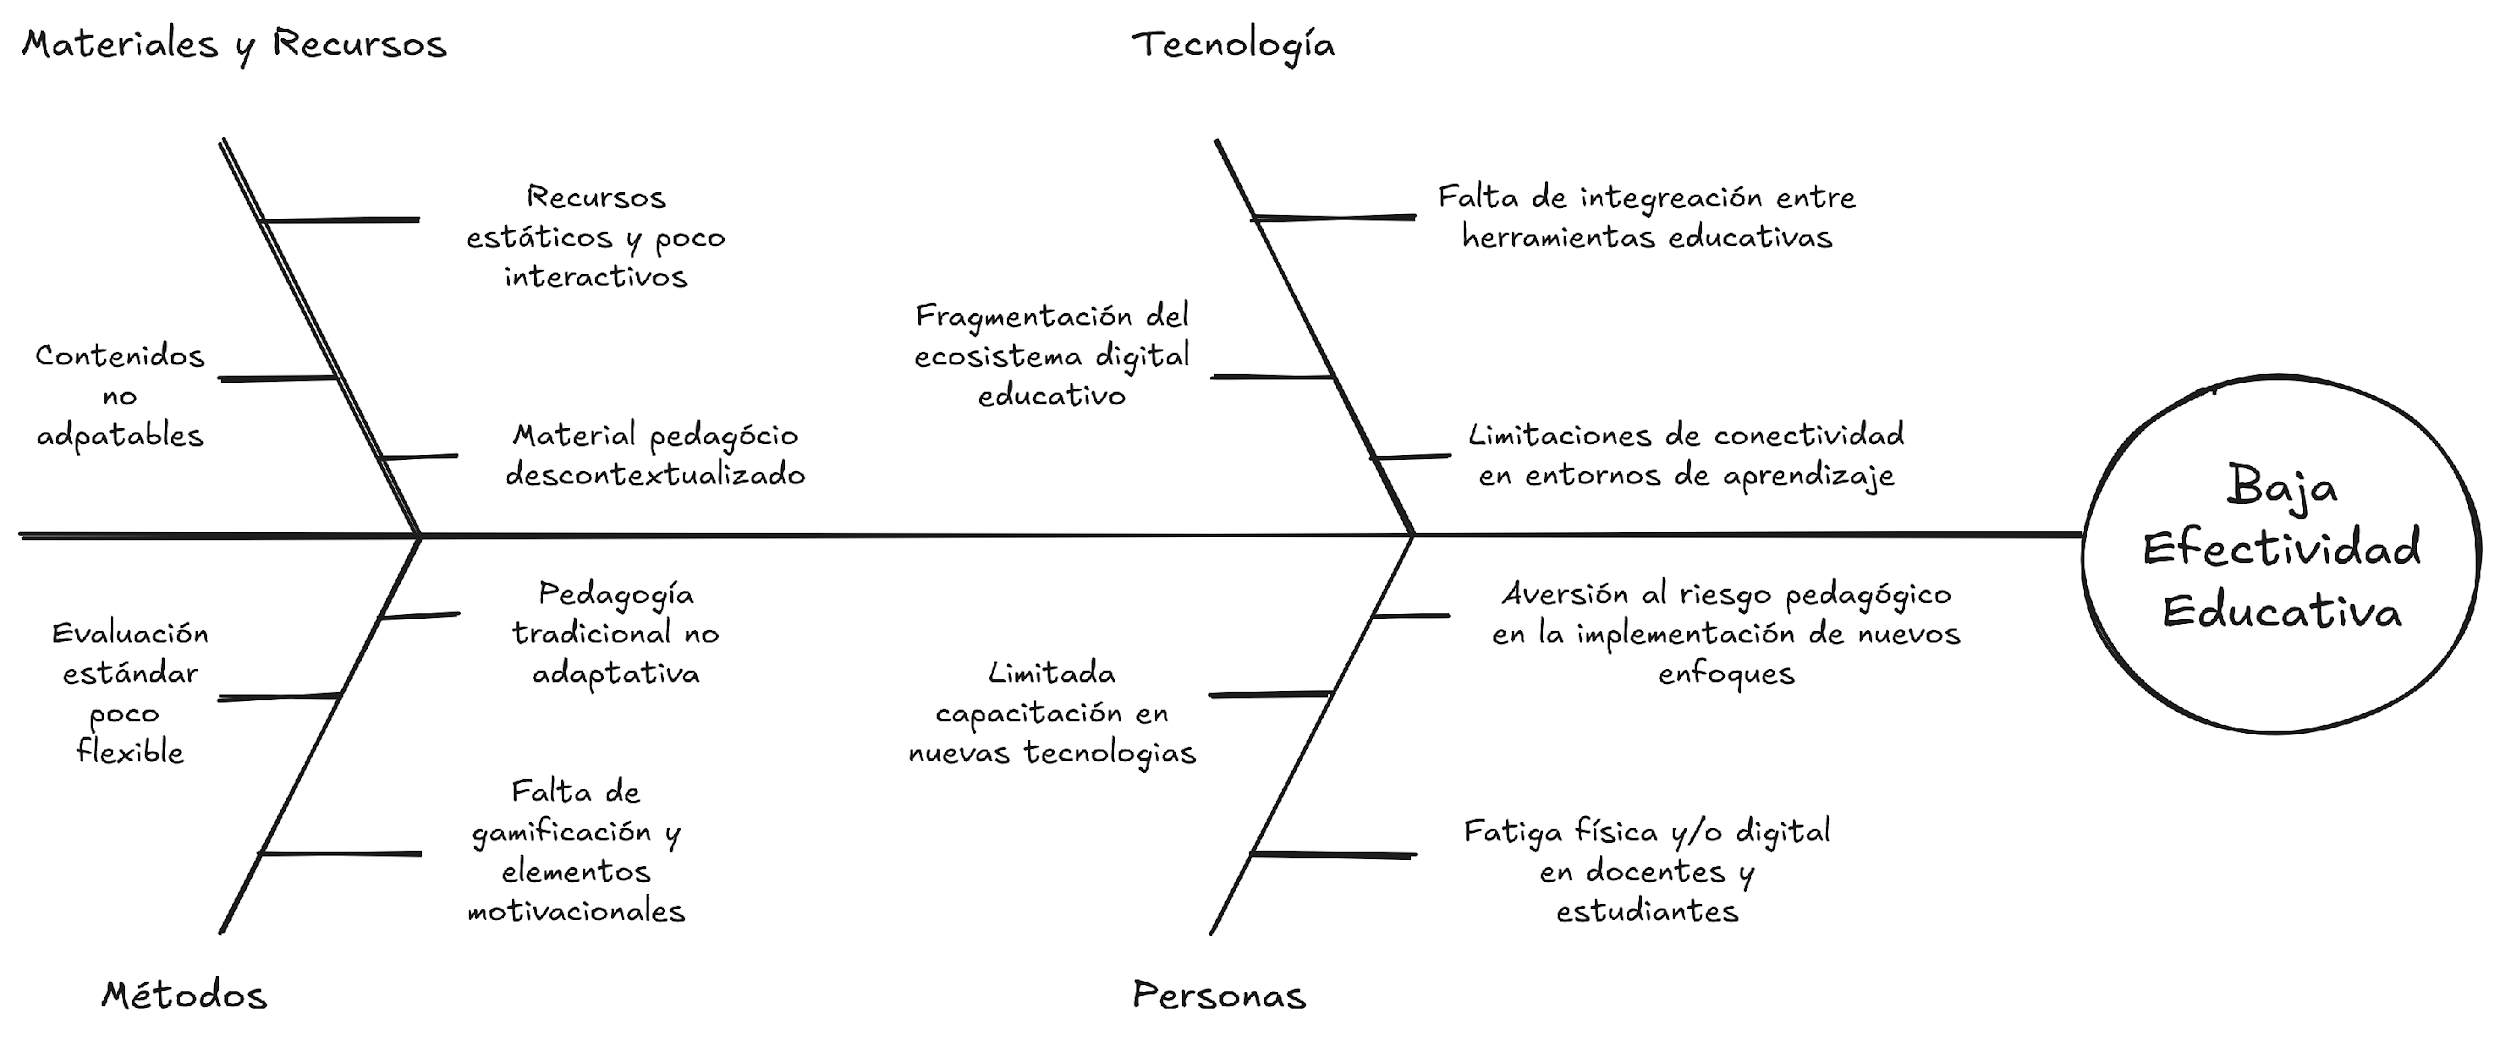
\includegraphics[width=0.9\textwidth]{images/diagrama_de_ishikawa.png}
	\caption{Diagrama Ishikawa: Causas de ineficiencia en el sistema tradicional.}
	\label{fig:ishikawa}
\end{figure}

El diagrama de Ishikawa muestra de manera sistemática las múltiples causas que contribuyen a la ineficiencia del sistema educativo tradicional, categorizando los factores en aspectos metodológicos, tecnológicos, motivacionales y estructurales.

\subsubsection{Análisis de las Causas del Problema Educativo Actual}

\paragraph{CAUSA 1: Disponibilidad irrestricta de herramientas para atajos académicos}
El acceso inmediato y sin restricciones a motores de búsqueda, herramientas de inteligencia artificial generativa, y plataformas de resolución de tareas ha creado un entorno donde los estudiantes pueden obtener respuestas completas sin necesidad de procesar información o desarrollar habilidades de pensamiento crítico. Esta disponibilidad tecnológica, aunque potencialmente beneficiosa para el aprendizaje, se ha convertido en una barrera cuando se utiliza como sustituto del proceso de aprendizaje genuino \cite{saputra2025}.

\paragraph{CAUSA 2: Ausencia de metodologías que transformen herramientas digitales en facilitadores de aprendizaje}
Las metodologías educativas actuales no han evolucionado para integrar efectivamente las herramientas digitales disponibles como parte del proceso de aprendizaje. En lugar de diseñar experiencias que aprovechen estas tecnologías para profundizar la comprensión, las instituciones educativas mantienen enfoques tradicionales que no consideran el potencial educativo de las herramientas digitales, creando una desconexión entre la realidad tecnológica de los estudiantes y las expectativas académicas \cite{nurhayati2025}.

\paragraph{CAUSA 3: Falta de elementos motivadores intrínsecos en las tareas académicas}
Las actividades académicas tradicionales carecen de elementos que generen motivación intrínseca en los estudiantes. Sin componentes como desafíos progresivos, retroalimentación inmediata, reconocimiento de logros, o conexión clara con aplicaciones prácticas, los estudiantes no encuentran razones convincentes para involucrarse genuinamente con el contenido académico, lo que los lleva a buscar alternativas que les permitan cumplir con menor esfuerzo \cite{sappaile2024}.

\subsection{Objetivos del proyecto}

\subsubsection{Objetivo general}

Desarrollar una aplicación educativa 3D gamificada que transforme las herramientas digitales de atajos académicos en facilitadores genuinos del aprendizaje, incrementando la motivación intrínseca y el compromiso estudiantil con el contenido académico a través de experiencias de aprendizaje inmersivas y relevantes.

\subsubsection{Objetivos específicos}

\begin{itemize}
\item Diseñar y desarrollar un entorno virtual 3D inmersivo que convierta las tareas académicas tradicionales en experiencias de aprendizaje motivadoras y significativas, donde los estudiantes perciban la relevancia práctica del conocimiento adquirido.
\item Implementar mecanismos de gamificación que fomenten el uso productivo de herramientas digitales, transformándolas de atajos para aprobar en instrumentos que profundicen la comprensión y desarrollen habilidades de pensamiento crítico.
\item Crear un sistema de progresión y recompensas que genere motivación intrínseca hacia el aprendizaje, donde el proceso de adquirir conocimiento sea tan atractivo como obtener la calificación final.
\item Desarrollar integraciones con plataformas educativas existentes que permitan a los docentes crear experiencias de aprendizaje que aprovechen las herramientas digitales disponibles como parte integral del proceso educativo, no como sustitutos del mismo.
\end{itemize}

\subsection{Alcance de la solución}

La plataforma educativa interactiva 3D para la gamificación de tareas académicas abarca:

\paragraph{Componentes funcionales}

\begin{itemize}
\item Sistema de registro y autenticación segura para administradores, docentes y estudiantes, con diferentes niveles de acceso según rol y responsabilidades.
\item Entorno virtual 3D inmersivo que simula un mundo medieval, con personajes interactivos, escenarios dinámicos y elementos visuales atractivos que contextualizan las actividades educativas.
\item Módulo de creación y gestión de tareas gamificadas que permite a los docentes configurar actividades educativas como misiones, retos y aventuras dentro del entorno virtual.
\item Sistema de evaluación y retroalimentación inmediata que convierte la evaluación tradicional en un proceso dinámico y motivador integrado a la narrativa del entorno.
\item Sistema de recompensas y progresión que incentiva la participación constante y reconoce los logros académicos.
\item Sistema de notificaciones vía push, correo electrónico, Discord y dentro de la plataforma para mantener informados a todos los usuarios sobre nuevas tareas, plazos y eventos.
\end{itemize}

\section{CAPÍTULO II: Marco contextual}

\subsection{Descripción del entorno de aplicación}

El proyecto se enfoca en contextos educativos secundarios, institucionales y universitarios donde los estudiantes han desarrollado patrones de comportamiento académico caracterizados por la búsqueda de aprobación sin compromiso real con el conocimiento \cite{academic_shortcuts2023,bretag2019}. A través de mecánicas de juego, progresión de habilidades y experiencias inmersivas en un entorno virtual medieval, la plataforma busca generar motivación intrínseca hacia el aprendizaje y revertir la percepción de irrelevancia que los estudiantes tienen sobre las tareas académicas.

\subsubsection{Gamificación Educativa}

La gamificación se define como la destreza de obtener elementos atractivos que se encuentran típicamente en los juegos y aplicarlos cuidadosamente en actividades productivas o del mundo real \cite{deterding2011}. Esta técnica ha ganado relevancia en diversos campos como la educación, el marketing y los entornos laborales, debido a su capacidad de fomentar la motivación, el compromiso y la participación activa.

El presente estudio explora qué hace atractivos a los juegos, resaltando aspectos como recompensas, diversión, interactividad, narrativa o historia, competencia, superación de retos y desafíos y posibilidad de compartir con amigos. Estos elementos, al ser incorporados estratégicamente en entornos no lúdicos, contribuyen a mejorar la experiencia del usuario y alcanzar objetivos específicos.

Contrario a lo que se podría pensar, las técnicas de gamificación no son recientes. Ya en el Imperio Romano existía un sistema de recompensas militares denominado Dona Militaria, el cual otorgaba distinciones como la Corona Cívica, por salvar la vida de un ciudadano, o la Corona Muralis, entregada al primer soldado que escalaba las murallas de una fortaleza enemiga, a pesar del alto riesgo de muerte \cite{polybius_histories}. Estos sistemas evidencian la existencia temprana de elementos como: feedback, insignias, competencia, colaboración, metas, niveles e interacción social.

Para comprender la gamificación en profundidad, es necesario distinguir entre los conceptos de juego y jugar. Jugar (Paidia) es una actividad espontánea, libre, sin finalidad concreta. Se asocia a la expresión creativa y la libertad de acción. Mientras que, Juego (Ludus): Actividad estructurada, con objetivos claros y reglas definidas. Implica una actitud deliberada de participación \cite{huizinga1938,caillois1961}.

La llamada actitud lúdica, conceptualizada por Friedrich Schiller \cite{schiller1795}, implica que los participantes se adhieren voluntariamente a las reglas del juego, le otorgan significado y están dispuestos a superar obstáculos innecesarios. En la gamificación, el desafío es lograr que el participante se acerque lo más posible al llamado "Círculo Mágico" del juego, donde se produce una inmersión total y significativa que potencia la motivación y la respuesta positiva ante los incentivos.

\paragraph{Modelo de Elementos de Gamificación}
Uno de los modelos más representativos para estructurar los elementos de la gamificación es la Pirámide de elementos \cite{werbach2012}, la cual se compone de tres niveles:

\begin{itemize}
\item \textbf{Dinámicas}: Son factores de diseño fundamentales relacionados con la naturaleza humana, como estatus, recompensa, competencia, altruismo, logro, emoción, progresión, relaciones y narrativa. Son universales e independientes del contexto cultural o demográfico.
\item \textbf{Mecánicas}: Son las reglas y sistemas que guían las acciones dentro de la experiencia gamificada, promoviendo el disfrute y el compromiso. Incluyen restricciones, desafíos, cooperación, retroalimentación y estrategias de progresión.
\item \textbf{Componentes}: Son elementos concretos y visibles, tales como logros, avatares, insignias, tablas de posiciones, puntos, equipos, niveles, objetos virtuales, recompensas y contenido desbloqueable.
\end{itemize}

\paragraph{Tipología de Jugadores}
Richard Bartle \cite{bartle1996} propuso una tipología de jugadores según su orientación hacia la acción o la interacción, y según el foco en el entorno o en los demás:

\begin{itemize}
\item \textbf{Triunfadores}: Están enfocados en progresar y dominar el entorno.
\item \textbf{Asesinos}: Buscan competir o dominar a otros jugadores.
\item \textbf{Exploradores}: Interesados en descubrir y comprender el mundo del juego.
\item \textbf{Socializadores}: Disfrutan de la interacción con otros participantes.
\end{itemize}

\paragraph{Misión}
Transformar las herramientas digitales de atajos académicos en facilitadores genuinos del aprendizaje mediante una plataforma 3D inmersiva que gamifica el proceso de enseñanza-aprendizaje, generando motivación intrínseca hacia el conocimiento y revertiendo patrones de comportamiento académico superficial a través de un mundo virtual medieval que convierte las tareas educativas en experiencias de aprendizaje significativas.

\paragraph{Visión}
Ser la plataforma educativa 3D de referencia mundial que establezca un nuevo paradigma en la relación entre estudiantes, herramientas digitales y conocimiento, donde el proceso de aprender sea tan atractivo y rewarding como obtener la calificación final, transformando definitivamente el uso de la tecnología en contextos educativos.

\paragraph{Análisis FODA}
El análisis FODA identifica las fortalezas, oportunidades, debilidades y amenazas del proyecto de gamificación educativa, proporcionando una base estratégica para la toma de decisiones en el desarrollo e implementación de la solución.

\begin{figure}[H]
	\centering
	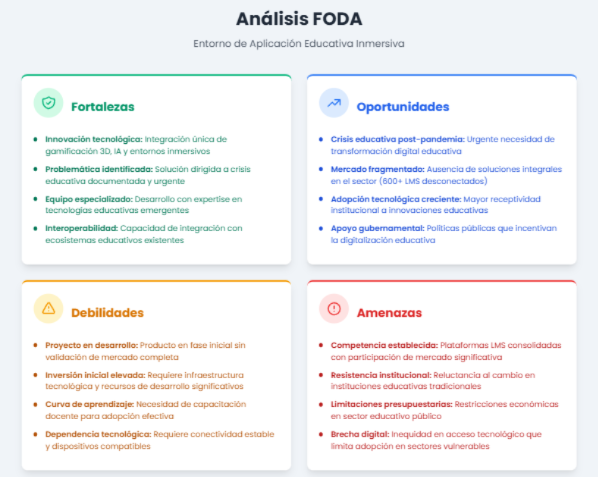
\includegraphics[width=0.9\textwidth]{images/analisis_foda.png}
	\caption{Análisis FODA del proyecto.}
	\label{fig:foda}
\end{figure}

\subsection{Fundamentos teóricos}

\subsubsection{Metodología de desarrollo de Software}

Una metodología para el desarrollo de software es un marco de trabajo que se usa para estructurar, planificar y controlar el proceso de desarrollo de sistemas de información \cite{velneo2023}.

\paragraph{Enfoque Ágil}
Las metodologías ágiles proporcionan una serie de pautas y principios junto a técnicas pragmáticas que hacen que la entrega del proyecto sea menos complicada y más satisfactoria tanto para los clientes como para los equipos de trabajo \cite{mayda2015}.

\myparagraph{Metodología Kanban}
La metodología Kanban es un marco ágil de flujo continuo que facilita la gestión visual del trabajo mediante un tablero y límites de trabajo en curso (WIP). Es especialmente adecuado para equipos pequeños y con disponibilidad limitada, ya que minimiza ceremonias formales y permite adaptar el flujo de trabajo a la capacidad real del equipo \cite{anderson2010}.

\subsubsection{Tecnologías de Desarrollo 3D}

\paragraph{Motores de renderizado 3D}
Los motores de renderizado 3D son frameworks que permiten crear, manipular y visualizar contenido tridimensional en aplicaciones web y móviles.

\myparagraph{Three.js}
Three.js es una biblioteca de JavaScript que abstrae WebGL para crear y renderizar escenas 3D con geometrías, materiales, luces y cámaras \cite{threejs2023}.

\myparagraph{Unity WebGL}
Unity WebGL es una plataforma de desarrollo que permite exportar aplicaciones Unity para ejecutarse en navegadores web mediante WebAssembly \cite{unity2023}.

\myparagraph{Babylon.js}
Babylon.js es un motor 3D en tiempo real desarrollado por Microsoft que se ejecuta en navegadores web usando WebGL y WebXR \cite{microsoft2023}.

\subsubsection{Frameworks de Desarrollo Backend}

\paragraph{Node.js}
Node.js es un entorno de tiempo de ejecución de JavaScript open source y multiplataforma que se ejecuta del lado del servidor. Utiliza un modelo basado en eventos asíncronos que permite gestionar múltiples conexiones simultáneas de forma eficiente \cite{acibeiro2022}, ideal para manejar las interacciones en tiempo real del entorno gamificado.

\paragraph{Next.js (API routes)}
Next.js es el framework elegido para integrar frontend y backend en una sola aplicación \cite{nextjs_docs2024}. Mediante las API routes de Next.js (con TypeScript) se implementarán endpoints server-side que gestionan autenticación, lógica de misiones, evaluación y acceso a la base de datos. Esta aproximación simplifica el despliegue y el mantenimiento al unificar el repositorio, aprovechar ventajas de SSR/SSG y facilitar la integración entre la parte UI (React/Three.js) y la capa de datos.

\paragraph{Django}
Django es un framework de desarrollo para Python que se emplea para la creación de páginas web. Se trata de una herramienta de código abierto que facilita el desarrollo web mediante su arquitectura Model-View-Template \cite{fernandez2022}, proporcionando robustez para el manejo de datos educativos y perfiles de usuario.

\subsubsection{Frameworks de Desarrollo Frontend}

\paragraph{React}
ReactJS es una biblioteca de JavaScript para el desarrollo de aplicaciones móviles y web. Contiene una colección de fragmentos de código JavaScript reutilizables utilizados para crear interfaces de usuario llamadas componentes \cite{deyimar2023}, facilitando la creación de interfaces interactivas para la gestión de tareas gamificadas.

\paragraph{Vue.js}
Vue.js es un framework open source de JavaScript que permite construir interfaces de usuarios de forma sencilla. Su característica principal es el trabajo con componentes reutilizables \cite{garcia2019}, ideal para desarrollar paneles de control y dashboards de progreso estudiantil.

\paragraph{Angular}
Angular es un framework front-end desarrollado por Google, diseñado para la creación de aplicaciones web robustas y escalables. Utiliza TypeScript y se basa en una arquitectura de componentes \cite{roldan2020}, proporcionando estructura sólida para aplicaciones educativas complejas.

\paragraph{Next.js}
Next.js es un framework construido sobre React que facilita el renderizado híbrido (SSR/SSG), generación de páginas estáticas y enrutamiento automático \cite{nextjs_docs2024}. Ofrece optimizaciones de rendimiento, manejo de rutas y capacidades de API que son útiles para construir portales educativos, dashboards y páginas con requisitos SEO y carga rápida sin sacrificar la interactividad del frontend.

\paragraph{Expo}
Expo es una plataforma y conjunto de herramientas para desarrollar aplicaciones móviles con React Native de forma rápida y con menos configuración \cite{expo_docs2023}. Permite prototipado ágil, despliegues OTA (over-the-air) y compatibilidad con Expo Go para pruebas en dispositivos reales, lo que facilita construir versiones móviles de la plataforma educativa para estudiantes y docentes.

\subsubsection{Sistemas de Base de Datos}

\paragraph{PostgreSQL}
PostgreSQL es un sistema de gestión de bases de datos relacional de código abierto que proporciona soporte para transacciones ACID, escalabilidad y extensibilidad. Ofrece características avanzadas como procedimientos almacenados y tipos de datos personalizados \cite{postgresql2024}, ideal para mantener la integridad de los datos educativos y el progreso estudiantil.

\paragraph{MongoDB}
MongoDB es una base de datos NoSQL orientada a documentos que almacena datos en formato JSON-like (BSON). Es especialmente útil para aplicaciones que requieren flexibilidad en el esquema de datos y escalabilidad horizontal \cite{mongodb2023}, permitiendo almacenar configuraciones dinámicas de misiones y logros estudiantiles.

\subsubsection{ORM}
\paragraph{Prisma}
Prisma es una opción  para interactuar con PostgreSQL desde las API routes de Next.js \cite{prisma_docs2024}. Ofrece tipado fuerte (TypeScript), generación automática de cliente, migraciones controladas y una DX (developer experience) que acelera el desarrollo. Prisma facilita modelar entidades como Usuarios, Misiones, Evaluaciones y Progreso y se integra bien con pruebas y despliegues.

\paragraph{Sequelize}
Sequelize es un ORM maduro para Node.js que soporta múltiples bases de datos SQL \cite{sequelize_docs2023}. Proporciona un API flexible, asociaciones explícitas y migraciones. Es una opción viable cuando se requiere compatibilidad con proyectos existentes en JavaScript puro o cuando se necesita un control granular de las consultas SQL.

\paragraph{TypeORM}
TypeORM es un ORM orientado a TypeScript que ofrece un enfoque tradicional basado en decoradores y entidades \cite{typeorm_docs2022}. Es útil en proyectos que prefieren una capa de abstracción con sintaxis declarativa y tiene buen soporte para patrones DDD (Domain-Driven Design). Sin embargo, su performance y DX pueden ser menos modernas que las de Prisma en ciertos flujos de trabajo.

\subsubsection{Plataformas de Despliegue}

\paragraph{Docker}
Docker es una plataforma de contenerización que empaqueta aplicaciones y sus dependencias en contenedores ligeros, garantizando portabilidad y consistencia entre entornos de desarrollo, pruebas y producción \cite{docker2023}. Facilita el despliegue de la aplicación educativa en diferentes instituciones.

\paragraph{Kubernetes}
Kubernetes es una plataforma de orquestación de contenedores que automatiza el despliegue, escalado y gestión de aplicaciones contenerizadas, proporcionando alta disponibilidad y recuperación automática \cite{kubernetes2023}. Permite manejar múltiples instancias concurrentes del entorno virtual para diferentes instituciones educativas.

\subsection{2.3 Descripción de los interesados del proyecto}

Los principales interesados del proyecto incluyen:

\begin{itemize}
	\item \textbf{Estudiantes}: Usuarios finales que interactuarán con la plataforma gamificada. Son el grupo objetivo principal y su adopción determinará el impacto pedagógico.
	\item \textbf{Docentes}: Creadores de contenido y evaluadores del proceso educativo. Diseñan las tareas, evalúan el rendimiento y configuran mecánicas y recompensas.
	\item \textbf{Instituciones educativas}: Adoptantes de la solución tecnológica. Se encargan de la implementación organizacional, políticas y financiamiento.
	\item \textbf{Área de TI}: Responsables de la implementación y mantenimiento técnico, despliegue en contenedores, monitoreo y backups.
	\item \textbf{Organismos reguladores}: Entidades que supervisan el cumplimiento de estándares educativos, privacidad y protección de datos.
\end{itemize}

\subsection{2.4 Análisis de la solución}

\subsubsection{2.4.1 Evaluación de motores de renderizado 3D}
Para el desarrollo del entorno 3D inmersivo se evalúan tres alternativas: Three.js, Unity WebGL y Babylon.js. Se empleará el método Scoring \cite{belton2002} para determinar la mejor opción. Este método de análisis multicriterio permite evaluar alternativas asignando ponderaciones a criterios relevantes y puntuaciones de satisfacción a cada opción, calculando un puntaje total que facilita la toma de decisiones objetivas.

\paragraph{Objetivo}
Seleccionar la mejor herramienta para el desarrollo del entorno 3D.

\paragraph{Alternativas}
Three.js, Unity WebGL, Babylon.js.

\paragraph{Criterios de evaluación}
Facilidad de uso, rendimiento, compatibilidad web, soporte de comunidad.
% A continuación se muestran las tablas de ponderación y satisfacción para la evaluación de motores 3D:
% Tabla 1
\begin{table}[ht]
\centering
\caption{Ponderación de los criterios motores de renderizado 3D (Valores asignados por el autor siguiendo metodología Scoring; ver \cite{belton2002})}
\begin{tabular}{l c}
\hline
Criterios & Ponderación \\
\hline
Facilidad de uso & 4 \\
Rendimiento & 5 \\
Compatibilidad web & 5 \\
Soporte de comunidad & 4 \\
\hline
\end{tabular}
\end{table}

% Tabla 2
\begin{table}[ht]
\centering
\caption{Nivel de satisfacción motores de renderizado 3D (Estimaciones del autor basadas en documentación técnica)}
\begin{tabular}{l c c c}
\hline
Criterios & Three.js & Unity WebGL & Babylon.js \\
\hline
Facilidad de uso & 8 & 6 & 7 \\
Rendimiento & 7 & 9 & 8 \\
Compatibilidad web & 9 & 7 & 8 \\
Soporte de comunidad & 9 & 8 & 6 \\
\hline
\end{tabular}
\end{table}
\FloatBarrier

% Tabla 3
\begin{table}[ht]
\centering
\caption{Comparación de motores de renderizado 3D}
\begin{tabular}{l c c c c}
\hline
Criterios & Ponderación & Three.js & Unity WebGL & Babylon.js \\
\hline
Facilidad de uso & 4 & 8 & 6 & 7 \\
Rendimiento & 5 & 7 & 9 & 8 \\
Compatibilidad web & 5 & 9 & 7 & 8 \\
Soporte de comunidad & 4 & 9 & 8 & 6 \\
\hline
Puntaje & - & 148 & 134 & 139 \\
\hline
\end{tabular}
\end{table}
\FloatBarrier
% --- Resultado para motores 3D (colocado después de sus tablas) ---
\subsubsection{2.4.1.1 Resultado de análisis de motores de renderizado 3D}
Considerando los resultados del método Scoring \cite{belton2002}, Three.js \cite{threejs2023} es la mejor opción para el desarrollo del entorno 3D debido a su excelente compatibilidad web, amplio soporte de comunidad y facilidad de integración con tecnologías web estándar.

% --- Evaluación de frameworks backend (descripción antes de tablas) ---
\subsubsection{2.4.2 Evaluación de frameworks backend}
Se evalúan tres frameworks para el desarrollo del backend: Node.js con NestJS, Django y Express.js.

\paragraph{Criterios de evaluación}
Escalabilidad, facilidad de desarrollo, rendimiento, ecosistema.
% A continuación se muestran las tablas de ponderación y satisfacción para la evaluación de frameworks backend:
% Tabla 4
\begin{table}[ht]
\centering
\caption{Ponderación de los criterios frameworks backend (Valores asignados por el autor siguiendo metodología Scoring; ver \cite{belton2002})}
\begin{tabular}{l c}
\hline
Criterios & Ponderación \\
\hline
Escalabilidad & 5 \\
Facilidad de desarrollo & 4 \\
Rendimiento & 5 \\
Ecosistema & 4 \\
\hline
\end{tabular}
\end{table}
\FloatBarrier

% Tabla 5
\begin{table}[ht]
\centering
\caption{Nivel de satisfacción frameworks backend (Estimaciones del autor basadas en documentación técnica)}
\begin{tabular}{l c c c}
\hline
Criterios & NestJS & Django & Express.js \\
\hline
Escalabilidad & 9 & 7 & 6 \\
Facilidad de desarrollo & 8 & 9 & 7 \\
Rendimiento & 8 & 6 & 8 \\
Ecosistema & 8 & 8 & 9 \\
\hline
\end{tabular}
\end{table}
\FloatBarrier

% Tabla 6
\begin{table}[ht]
\centering
\caption{Comparación de frameworks backend}
\begin{tabular}{l c c c c}
\hline
Criterios & Ponderación & NestJS & Django & Express.js \\
\hline
Escalabilidad & 5 & 9 & 7 & 6 \\
Facilidad de desarrollo & 4 & 8 & 9 & 7 \\
Rendimiento & 5 & 8 & 6 & 8 \\
Ecosistema & 4 & 8 & 8 & 9 \\
\hline
Puntaje & - & 149 & 126 & 132 \\
\hline
\end{tabular}
\end{table}
\FloatBarrier
% --- Resultado para frameworks backend (colocado después de sus tablas) ---
\subsubsection{2.4.2.1 Resultado de análisis de frameworks backend}
NestJS obtiene la mejor puntuación debido a su arquitectura modular, excelente escalabilidad y integración nativa con TypeScript, lo que facilita el desarrollo de APIs robustas para la aplicación educativa.

% --- Evaluación de frameworks frontend (descripción antes de tablas) ---
\subsubsection{2.4.3 Evaluación de frameworks frontend}
Se evalúan tres frameworks (y alternativas relacionadas) para el desarrollo del frontend: React, Vue.js, Angular, Next.js y Expo.

\paragraph{Criterios de evaluación}
Curva de aprendizaje, rendimiento, ecosistema, integración 3D.
% A continuación se muestran las tablas de ponderación y satisfacción para la evaluación de frameworks frontend:
% Tabla 7
\begin{table}[ht]
\centering
\caption{Ponderación de los criterios frameworks frontend (Valores asignados por el autor siguiendo metodología Scoring; ver \cite{belton2002})}
\begin{tabular}{l c}
\hline
Criterios & Ponderación \\
\hline
Curva de aprendizaje & 4 \\
Rendimiento & 5 \\
Ecosistema & 4 \\
Integración 3D & 5 \\
\hline
\end{tabular}
\end{table}
\FloatBarrier

% Tabla 8
\begin{table}[ht]
\centering
\caption{Nivel de satisfacción frameworks frontend (Estimaciones del autor basadas en documentación técnica)}
\begin{tabular}{l c c c c c}
\hline
Criterios & React & Vue.js & Angular & Next.js & Expo \\
\hline
Curva de aprendizaje & 7 & 9 & 5 & 7 & 8 \\
Rendimiento & 8 & 8 & 7 & 9 & 6 \\
Ecosistema & 9 & 7 & 8 & 9 & 6 \\
Integración 3D & 9 & 6 & 7 & 9 & 5 \\
\hline
\end{tabular}
\end{table}
\FloatBarrier

% Tabla 9
\begin{table}[ht]
\centering
\caption{Comparación de frameworks frontend}
\begin{tabular}{l c c c c c c}
\hline
Criterios & Ponderación & React & Vue.js & Angular & Next.js & Expo \\
\hline
Curva de aprendizaje & 4 & 7 & 9 & 5 & 6 & 8 \\
Rendimiento & 5 & 8 & 8 & 7 & 9 & 6 \\
Ecosistema & 4 & 9 & 7 & 8 & 8 & 6 \\
Integración 3D & 5 & 9 & 6 & 7 & 9 & 5 \\
\hline
Puntaje & - & 149 & 134 & 122 & 154 & 111 \\
\hline
\end{tabular}
\end{table}
\FloatBarrier
% --- Resultado para frameworks frontend (colocado después de sus tablas) ---
\subsubsection{2.4.3.1 Resultado de análisis de frameworks frontend}
Según los resultados del análisis multicriterio \cite{belton2002}, Next.js \cite{nextjs_docs2024} es la opción recomendada para el frontend en este proyecto debido a su excelente integración con bibliotecas 3D (cuando se usa junto a React/Three.js), sus capacidades de renderizado híbrido (SSR/SSG), y sus optimizaciones de rendimiento para páginas con requisitos SEO y cargas iniciales rápidas. React sigue siendo una opción sólida y más generalista, pero en función de los criterios y ponderaciones utilizadas, Next.js obtiene el puntaje más alto. Expo \cite{expo_docs2023} mantiene utilidad para prototipado y versiones móviles, pero queda por detrás en la integración 3D.

% --- Evaluación de sistemas de base de datos (descripción antes de tablas) ---
\subsubsection{2.4.4 Evaluación de sistemas de base de datos}
Se evalúan dos sistemas de base de datos: PostgreSQL y MongoDB.

\paragraph{Criterios de evaluación}
Consistencia de datos, escalabilidad, facilidad de uso, soporte.
% A continuación se muestran las tablas de ponderación y satisfacción para la evaluación de sistemas de base de datos:
% Tabla 10
\begin{table}[ht]
\centering
\caption{Ponderación de los criterios sistemas de base de datos (Valores asignados por el autor siguiendo metodología Scoring; ver \cite{belton2002})}
\begin{tabular}{l c}
\hline
Criterios & Ponderación \\
\hline
Consistencia de datos & 5 \\
Escalabilidad & 4 \\
Facilidad de uso & 4 \\
Soporte & 3 \\
\hline
\end{tabular}
\end{table}

% Tabla 11
\begin{table}[ht]
\centering
\caption{Nivel de satisfacción sistemas de base de datos (Estimaciones del autor basadas en documentación técnica)}
\begin{tabular}{l c c}
\hline
Criterios & PostgreSQL & MongoDB \\
\hline
Consistencia de datos & 9 & 6 \\
Escalabilidad & 7 & 9 \\
Facilidad de uso & 7 & 8 \\
Soporte & 9 & 7 \\
\hline
\end{tabular}
\end{table}

% Tabla 12
\begin{table}[ht]
\centering
\caption{Comparación de sistemas de base de datos}
\begin{tabular}{l c c c}
\hline
Criterios & Ponderación & PostgreSQL & MongoDB \\
\hline
Consistencia de datos & 5 & 9 & 6 \\
Escalabilidad & 4 & 7 & 9 \\
Facilidad de uso & 4 & 7 & 8 \\
Soporte & 3 & 9 & 7 \\
\hline
Puntaje & - & 134 & 118 \\
\hline
\end{tabular}
\end{table}

\subsubsection{2.4.4.1 Resultado de análisis de sistemas de base de datos}
PostgreSQL es la mejor opción debido a su robustez, consistencia de datos mediante transacciones ACID y excelente soporte para datos relacionales complejos necesarios en un sistema educativo.

% --- Evaluación de ORMs (descripción antes de tablas) ---
\subsubsection{2.4.5 Evaluación de ORM}
Se evalúan tres ORMs populares para integrar la capa de datos con las API routes de Next.js: Prisma, Sequelize y TypeORM. Se aplicará nuevamente el método Scoring \cite{belton2002} para comparar alternativas según criterios relevantes para este proyecto.

\paragraph{Criterios de evaluación}
Tipado/seguridad, facilidad de uso, rendimiento, migraciones y experiencia de desarrollador (DX).
% A continuación se muestran las tablas de ponderación y satisfacción para la evaluación de ORMs:
% Tabla 13
\begin{table}[ht]
\centering
\caption{Ponderación de los criterios ORMs (Valores asignados por el autor siguiendo metodología Scoring; ver \cite{belton2002})}
\begin{tabular}{l c}
\hline
Criterios & Ponderación \\
\hline
Tipado / Seguridad & 5 \\
Facilidad de uso & 4 \\
Rendimiento & 4 \\
Migraciones & 3 \\
Experiencia de desarrollador (DX) & 4 \\
\hline
\end{tabular}
\end{table}
\FloatBarrier

% Tabla 14
\begin{table}[ht]
\centering
\caption{Nivel de satisfacción ORMs (Estimaciones del autor basadas en documentación técnica)}
\begin{tabular}{l c c c}
\hline
Criterios & Prisma & Sequelize & TypeORM \\
\hline
Tipado / Seguridad & 9 & 6 & 8 \\
Facilidad de uso & 8 & 7 & 7 \\
Rendimiento & 8 & 7 & 7 \\
Migraciones & 8 & 7 & 6 \\
DX & 9 & 7 & 7 \\
\hline
\end{tabular}
\end{table}
\FloatBarrier

% Tabla 15
\begin{table}[ht]
\centering
\caption{Comparación de ORMs}
\begin{tabular}{l c c c c}
\hline
Criterios & Ponderación & Prisma & Sequelize & TypeORM \\
\hline
Tipado / Seguridad & 5 & 9 & 6 & 8 \\
Facilidad de uso & 4 & 8 & 7 & 7 \\
Rendimiento & 4 & 8 & 7 & 7 \\
Migraciones & 3 & 8 & 7 & 6 \\
DX & 4 & 9 & 7 & 7 \\
\hline
Puntaje & - &  \textendash &  \textendash &  \textendash \\
\hline
\end{tabular}
\end{table}
\FloatBarrier

% Calcular puntaje total (mostrado en texto para mantener el control en LaTeX)
\subsubsection{2.4.5.1 Resultado de análisis de ORMs}
Aplicando la matriz de ponderaciones y multiplicando por las puntuaciones de satisfacción (cada criterio sobre 10), se obtiene un puntaje aproximado (redondeado) que favorece a Prisma en este contexto de Next.js con TypeScript debido a su tipado fuerte, excelente DX y sistema de migraciones integrado \cite{prisma_docs2024,sequelize_docs2023,typeorm_docs2022}. Por tanto, se recomienda adoptar Prisma como ORM principal para la implementación de las API routes y la gestión de entidades como Usuarios, Misiones y Progreso.

\paragraph{Observaciones}
Prisma ofrece ventajas significativas en proyectos TypeScript por su cliente tipado, generación de tipos y migraciones declarativas. Sequelize sigue siendo una opción válida si se requiere compatibilidad con código JavaScript existente, mientras que TypeORM puede ser preferible en equipos que favorezcan un estilo declarativo con decoradores y entidades al estilo tradicional \cite{prisma_docs2024,sequelize_docs2023,typeorm_docs2022}.



\section{CAPÍTULO III: Propuesta de la solución}

\subsection{3.1 Descripción de la solución}
La solución propuesta consiste en el desarrollo de una aplicación educativa 3D que transforme la experiencia de aprendizaje tradicional mediante la gamificación de tareas académicas en un entorno virtual medieval inmersivo. El sistema integra tecnologías web modernas con estrategias pedagógicas innovadoras para crear un ecosistema educativo que incremente la motivación estudiantil y mejore los resultados de aprendizaje.

La aplicación funcionará como una plataforma integral que conecta docentes, estudiantes y administradores a través de una interfaz web responsiva y aplicaciones móviles. El entorno virtual 3D, desarrollado con Three.js, simula un mundo medieval donde las actividades académicas se transforman en misiones, aventuras y desafíos interactivos que mantienen el engagement estudiantil mientras refuerzan competencias académicas específicas.

El backend se implementará utilizando las API routes de Next.js (con TypeScript) como capa de servidor integrada en la misma aplicación, aprovechando el renderizado híbrido y las ventajas de un único repositorio para cliente y servidor. Estas rutas proporcionarán endpoints para autenticación, administración de usuarios, creación de contenidos gamificados, sistema de evaluaciones y análisis de progreso estudiantil. La base de datos PostgreSQL garantizará la integridad y consistencia de la información educativa, mientras que las integraciones con plataformas existentes como Canvas y Discord ampliarán las capacidades del ecosistema.

\subsubsection{3.1.1 Diagrama de arquitectura}
En el siguiente diagrama se define la arquitectura del proyecto. Se detallan las herramientas empleadas: en el backend, NestJS con TypeScript; en el lado del cliente, React con Three.js para el entorno 3D; como base de datos, PostgreSQL desplegado en servicios cloud (AWS); seguridad mediante JWT integrado con NestJS Guards y autenticación OAuth2 con correo institucional (Google/Microsoft). El sistema incluye integraciones con Canvas LMS y Discord para comunicación, así como un servicio de notificaciones push.

\begin{figure}[H]
	\centering
	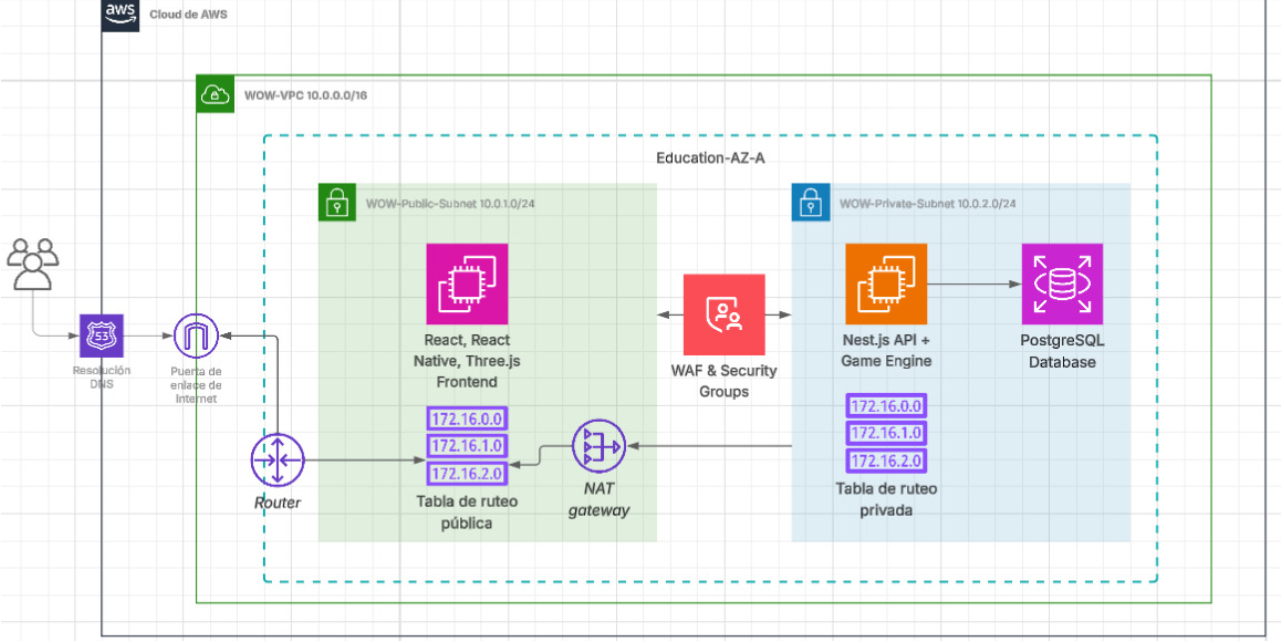
\includegraphics[width=0.95\textwidth]{images/arquitectura.png}
	\caption{Diagrama de arquitectura del proyecto.}
	\label{fig:arquitectura}
\end{figure}

\paragraph{Descripción de componentes principales}
\begin{itemize}
	\item \textbf{Cliente Web (React + Three.js dentro de Next.js)}: Interfaz principal para estudiantes y docentes. Renderiza el entorno 3D y gestiona interacción en tiempo real.
	\item \textbf{API Backend (Next.js API routes)}: Endpoints server-side integrados en Next.js que orquestan la lógica de negocio: autenticación, misiones, evaluación, recompensas y analítica básica.
	\item \textbf{Módulo de Autenticación}: OAuth2 (Google/Microsoft) + JWT (access/refresh) implementado mediante middleware y API routes de Next.js.
	\item \textbf{Base de Datos (PostgreSQL)}: Persistencia relacional: usuarios, cursos, misiones, evaluaciones, progreso, recompensas, avatares.
	\item \textbf{Integraciones Externas}: Canvas (importación/exportación de cursos y calificaciones), Discord (canales de comunicación), Servicio Push (notificaciones de eventos y misiones).
	\item \textbf{Servicio de Analítica}: Procesa eventos de interacción para generar métricas de engagement y rendimiento; puede ejecutarse en serverless functions o microservicios según carga.
	\item \textbf{Orquestación / Infraestructura}: Contenedores Docker para servicios auxiliares y despliegue en Vercel/Cloud (o Kubernetes) para la parte de backend/servicios. El almacenamiento y procesamiento en la nube se realiza exclusivamente en AWS.
\end{itemize}

\subsubsection{3.1.2 Diagramas de Procesos de Negocio (BPMN 2.0)}
Los diagramas BPMN representan el flujo operativo completo del sistema. Capturan la transformación digital de procesos educativos tradicionales, eliminando ineficiencias y habilitando trazabilidad.

\paragraph{Proceso 1: Gestión de Misiones Educativas}
\begin{figure}[H]
	\centering
	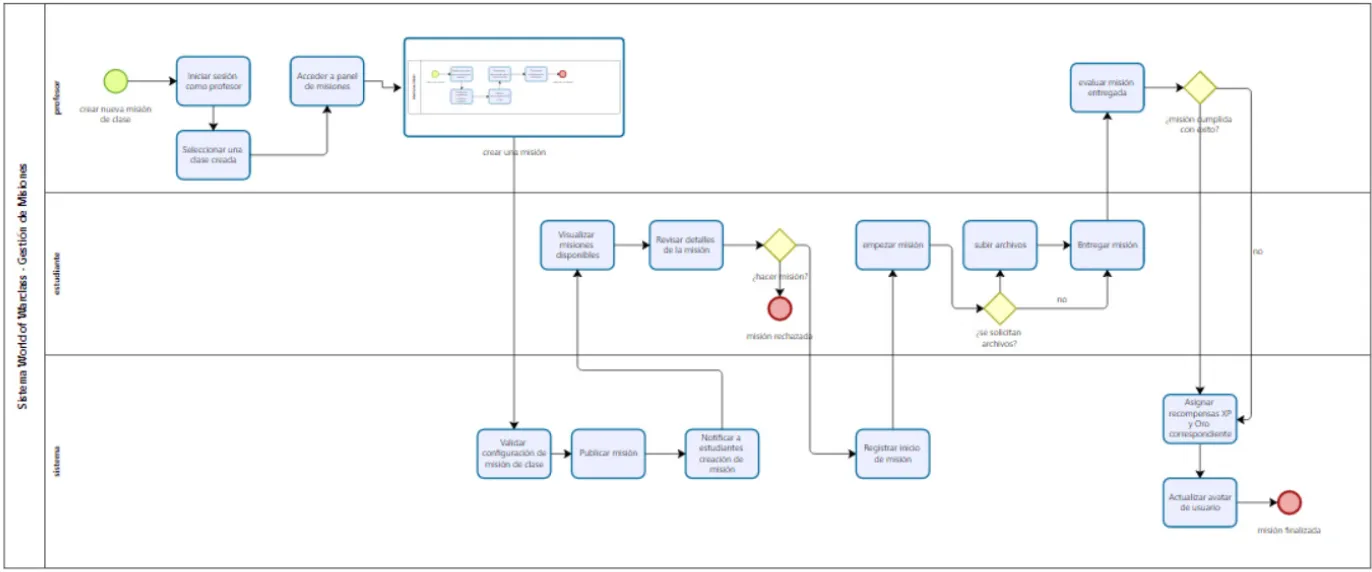
\includegraphics[width=0.95\textwidth]{images/bizgi_gestion_de_misiones.png}
	\caption{Modelo de proceso: Gestión de Misiones Educativas.}
	\label{fig:proc-misiones}
\end{figure}
\textit{Flujo}: Creación de misión (docente) $\rightarrow$ Definición de objetivos y recompensas $\rightarrow$ Publicación $\rightarrow$ Asignación automática/selección $\rightarrow$ Ejecución en entorno 3D $\rightarrow$ Evaluación $\rightarrow$ Retroalimentación y registro de progreso.

\paragraph{Proceso 2: Sistema de Evaluación Gamificada}
\begin{figure}[H]
	\centering
	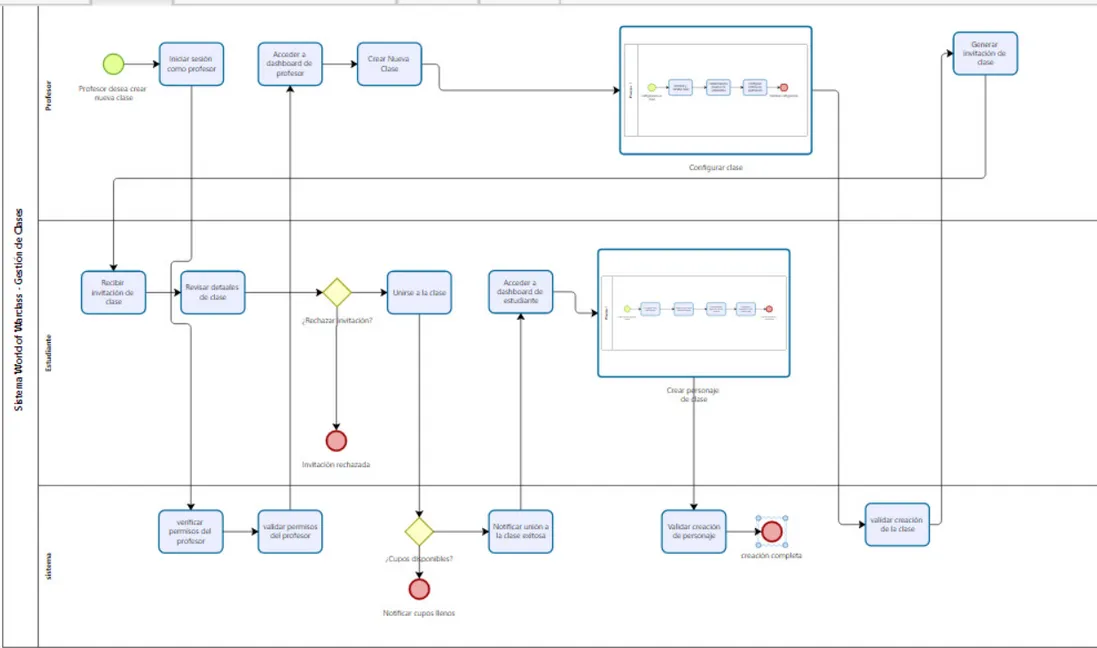
\includegraphics[width=0.95\textwidth]{images/bizagi_gestion_de_clases.png}
	\caption{Modelo de proceso: Sistema de Evaluación Gamificada.}
	\label{fig:proc-evaluacion}
\end{figure}
\textit{Flujo}: Participación estudiante $\rightarrow$ Recolección de métricas $\rightarrow$ Asignación de puntos y logros $\rightarrow$ Actualización de avatar/nivel $\rightarrow$ Registro en base de datos $\rightarrow$ Notificación a docente.

\paragraph{Proceso 3: Análisis y Seguimiento del Progreso}
\begin{figure}[H]
	\centering
	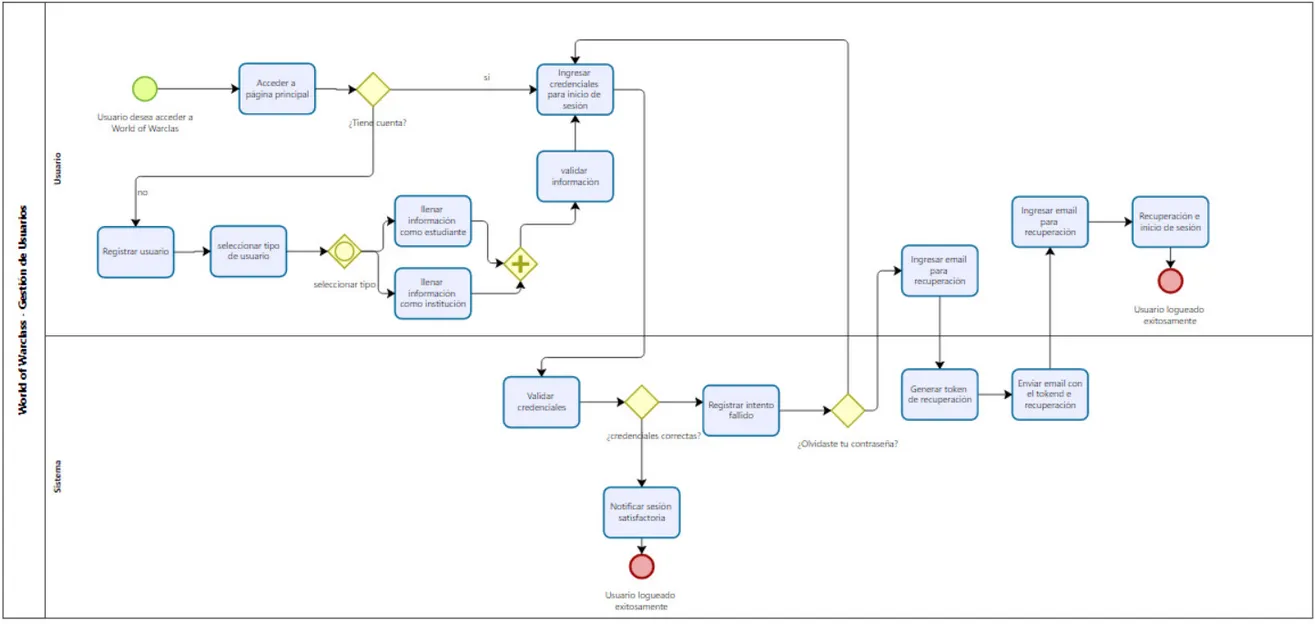
\includegraphics[width=0.95\textwidth]{images/bizagi_gestion_de_usuarios.png}
	\caption{Modelo de proceso: Análisis y Seguimiento del Progreso Estudiantil.}
	\label{fig:proc-analitica}
\end{figure}
\textit{Flujo}: Captura de eventos $\rightarrow$ Almacenamiento $\rightarrow$ Procesamiento analítico $\rightarrow$ Generación de paneles $\rightarrow$ Intervención pedagógica.

\subsubsection{3.1.3 Diagrama Entidad-Relación}
El modelo entidad-relación define las estructuras nucleares para garantizar integridad y trazabilidad.
\begin{figure}[H]
	\centering
	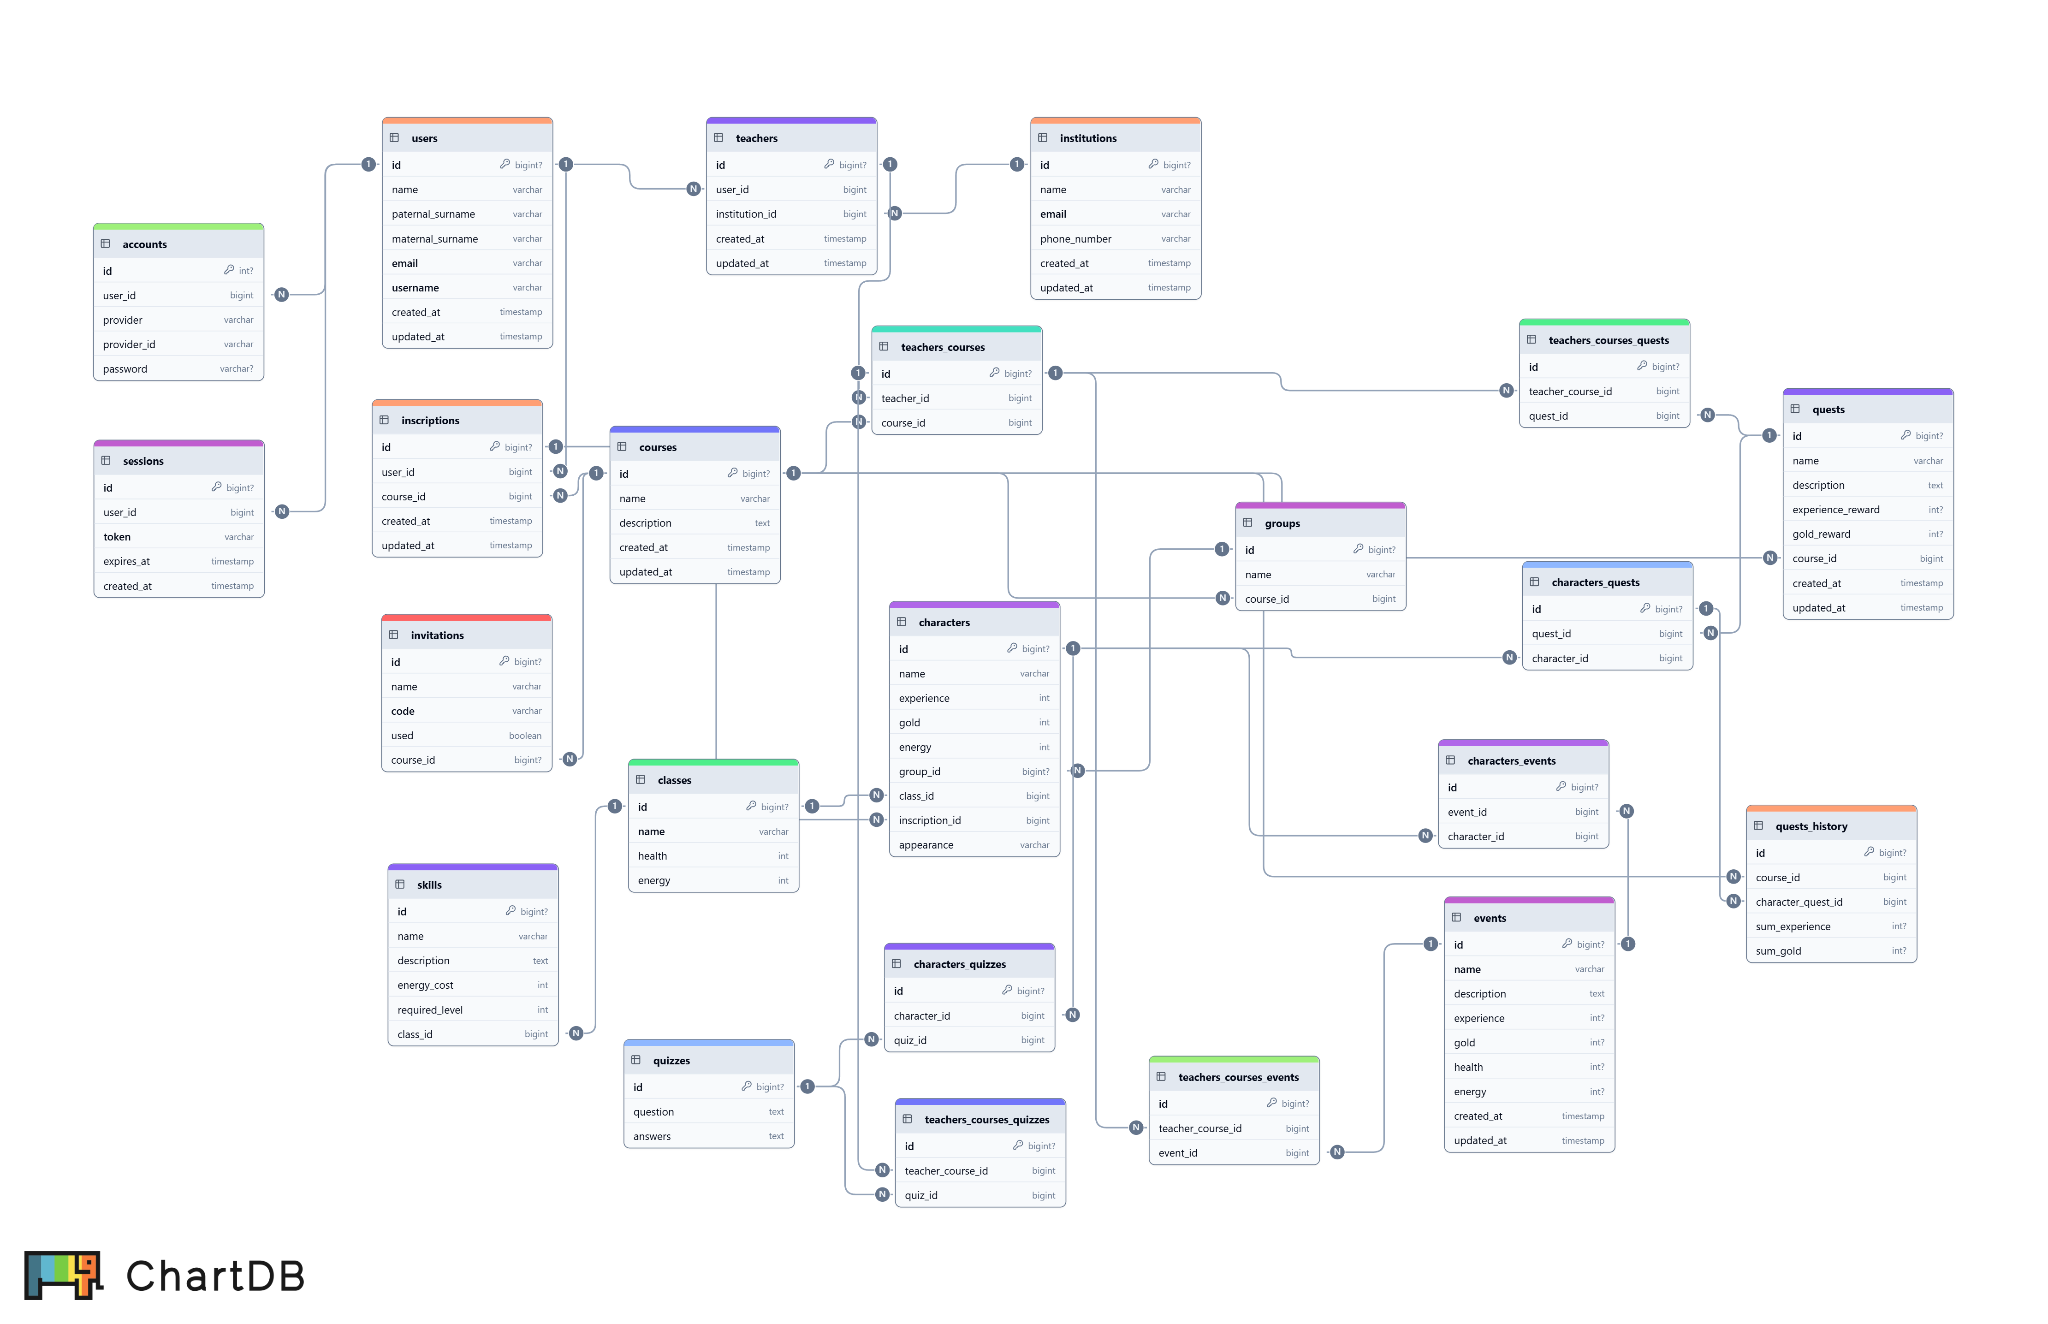
\includegraphics[width=0.95\textwidth]{images/mer.png}
	\caption{Diagrama entidad-relación del sistema.}
	\label{fig:der}
\end{figure}
Entidades principales: Usuarios, Instituciones, Cursos, Misiones, Evaluaciones, Progreso, Recompensas, Avatares. Relaciones jerárquicas permiten seguimiento académico personalizado.

\subsubsection{3.1.4 Prototipo de Interfaces (Figma)}
Las interfaces clave se diseñarán en Figma priorizando usabilidad y consistencia visual.
\begin{figure}[H]
	\centering
	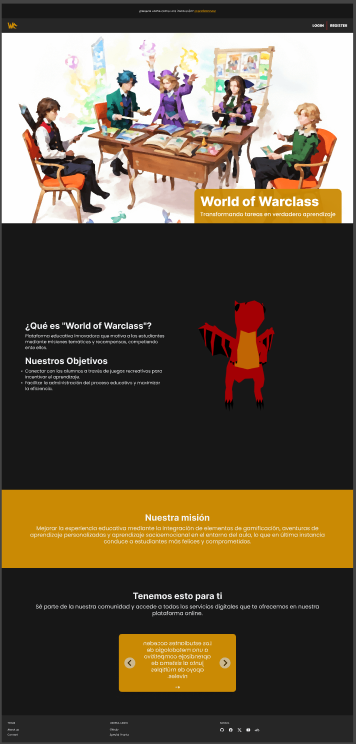
\includegraphics[width=0.75\textwidth]{images/pagina_web_inicio.png}
	\caption{Interfaz principal (home) para usuarios no autenticados.}
	\label{fig:ui-home}
\end{figure}
\begin{figure}[H]
	\centering
	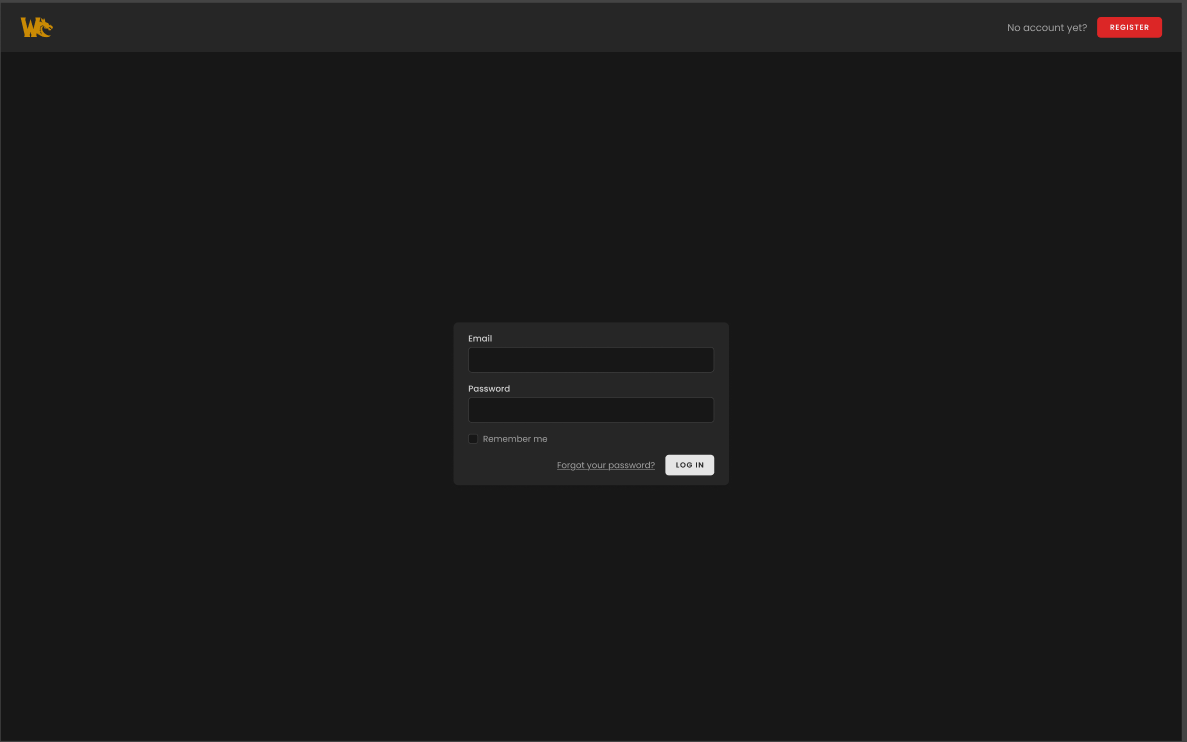
\includegraphics[width=0.75\textwidth]{images/pagina_web_iniciar-sesion.png}
	\caption{Interfaz de Autenticación del proyecto.}
	\label{fig:ui-login}
\end{figure}
\begin{figure}[H]
	\centering
	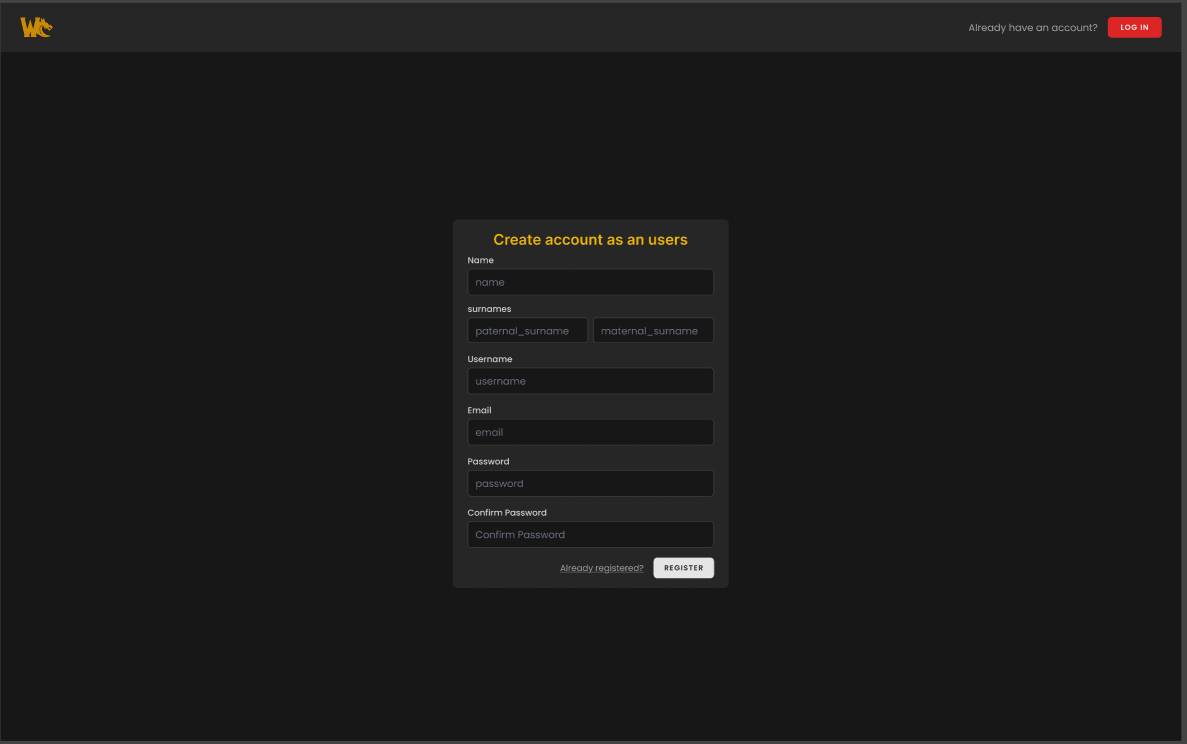
\includegraphics[width=0.75\textwidth]{images/pagina_web_registro.png}
	\caption{Interfaz de Registro de usuario del proyecto.}
	\label{fig:ui-register}
\end{figure}
\begin{figure}[H]
	\centering
	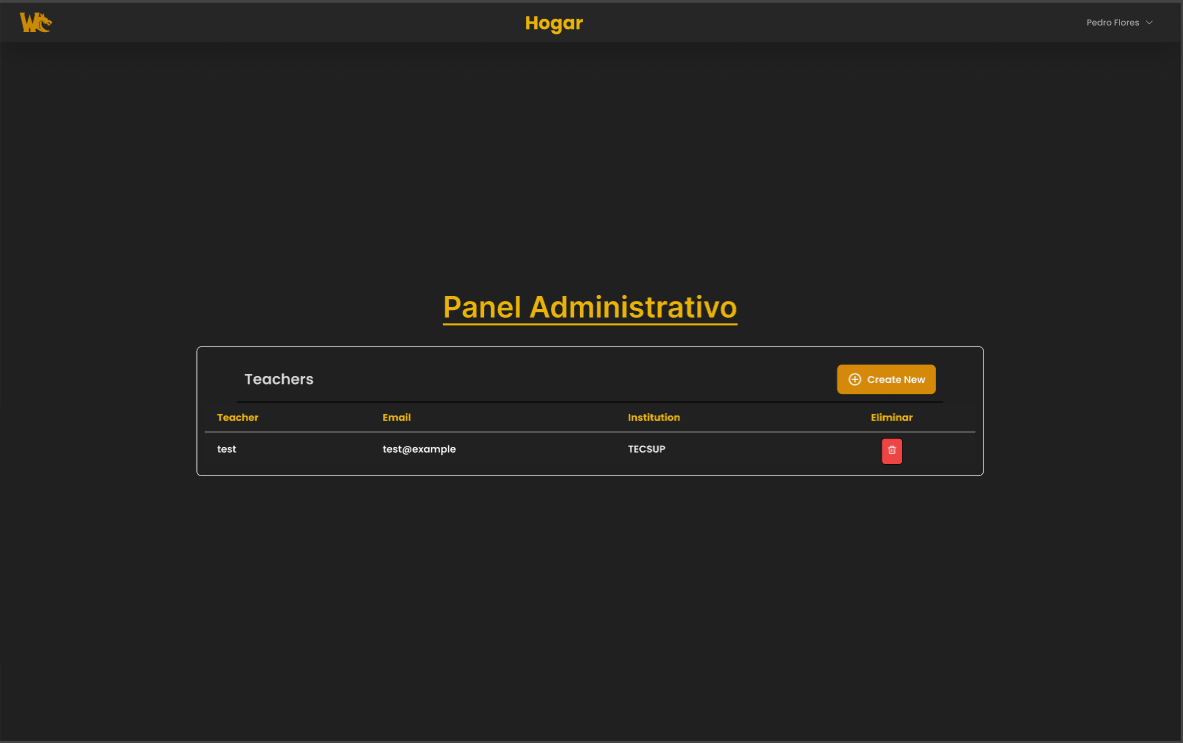
\includegraphics[width=0.75\textwidth]{images/pagina_web_panel-administrativo.png}
	\caption{Interfaz de panel de administración del profesor.}
	\label{fig:ui-profesor}
\end{figure}
\begin{figure}[H]
	\centering
	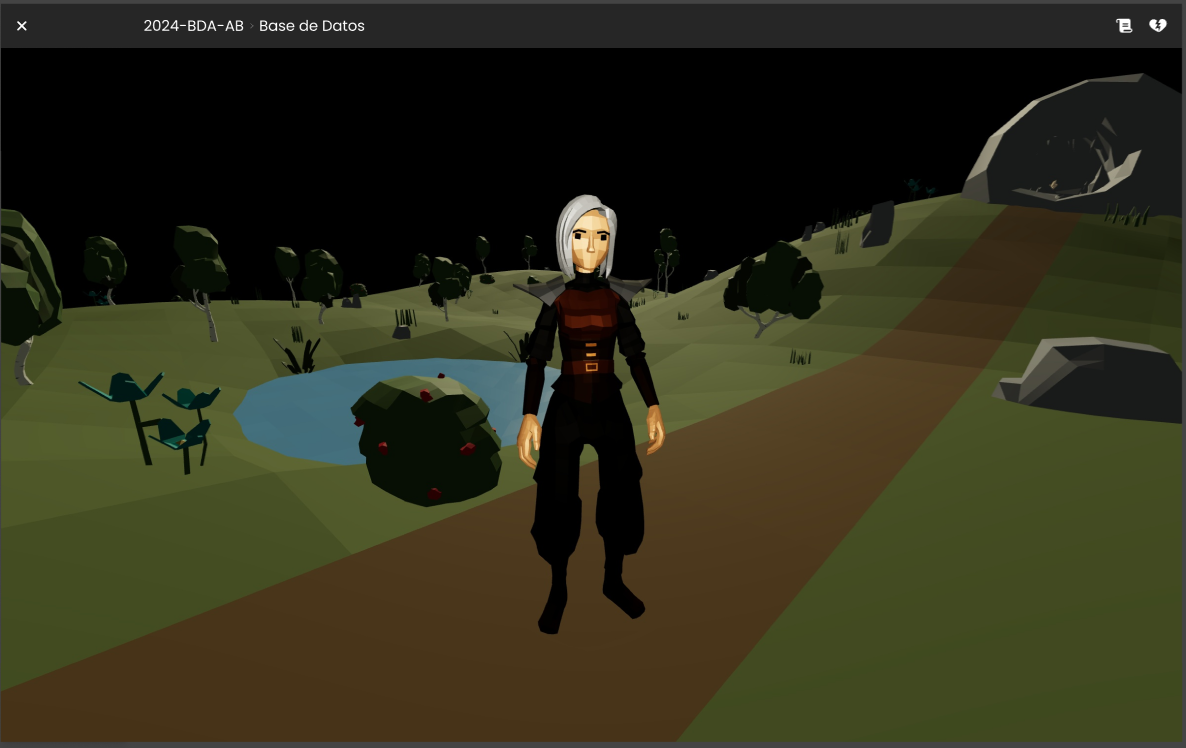
\includegraphics[width=0.75\textwidth]{images/pagina_web_vista-alumno.png}
	\caption{Gestión de avatar del estudiante.}
	\label{fig:ui-avatar}
\end{figure}

\subsection{3.2 Descripción de la metodología de desarrollo de software}
La metodología seleccionada para el proyecto es \textbf{Kanban} (marco ágil de flujo continuo) complementada con prácticas de integración continua y despliegue continuo (CI/CD). Se eligió debido a que el equipo es muy pequeño (2 personas) y varios integrantes trabajan en sus tiempos libres; Kanban reduce la sobrecarga de ceremonias y facilita el flujo de trabajo mediante un tablero visual y límites de trabajo en curso (WIP).

\subsubsection{3.2.1 Justificación de la selección de Kanban}
\begin{itemize}
	\item \textbf{Equipo pequeño y disponibilidad limitada}: con solo dos personas y trabajo a tiempo parcial, Kanban minimiza reuniones y coordinación pesada.
	\item \textbf{Flujo continuo}: permite priorizar y avanzar tareas según la capacidad real del equipo sin forzar iteraciones fijas.
	\item \textbf{Menor overhead administrativo}: no requiere ceremonias formales obligatorias (planning, sprint review, retro) lo que ahorra tiempo en proyectos con recursos limitados.
	\item \textbf{Visualización y control de WIP}: el tablero Kanban facilita identificar cuellos de botella, visualizar el progreso y limitar el trabajo en curso para mejorar el flujo.
\end{itemize}

\subsubsection{3.2.2 Épicas e Historias de Usuario}
Las épicas agrupan funcionalidades estratégicas. A continuación se muestran épicas con ejemplos de historias asociadas:

\begin{table}[ht]
	\centering
	\caption{Épicas e historias de usuario (Tabla 14).}
	\begin{tabular}{p{3cm} p{10cm}}
		\toprule
		Épica & Historias (resumen) \\
		\midrule
		Autenticación & Como estudiante quiero registrarme con mi cuenta institucional para acceder a mis cursos.\\
		Misiones & Como docente quiero crear una misión con objetivos y recompensas para motivar a mis alumnos.\\
		Evaluación & Como docente quiero ver el rendimiento agregado de una misión para ajustar la dificultad.\\
		Progreso & Como estudiante quiero visualizar mi nivel y logros para entender mi avance.\\
		Analítica & Como administrador quiero paneles de uso para evaluar adopción y engagement.\\
		Integraciones & Como docente quiero importar calificaciones desde Canvas para unificar seguimiento.\\
		Notificaciones & Como estudiante quiero recibir avisos cuando haya nuevas misiones disponibles.\\
		\bottomrule
	\end{tabular}
\end{table}

\begin{figure}[H]
	\centering
	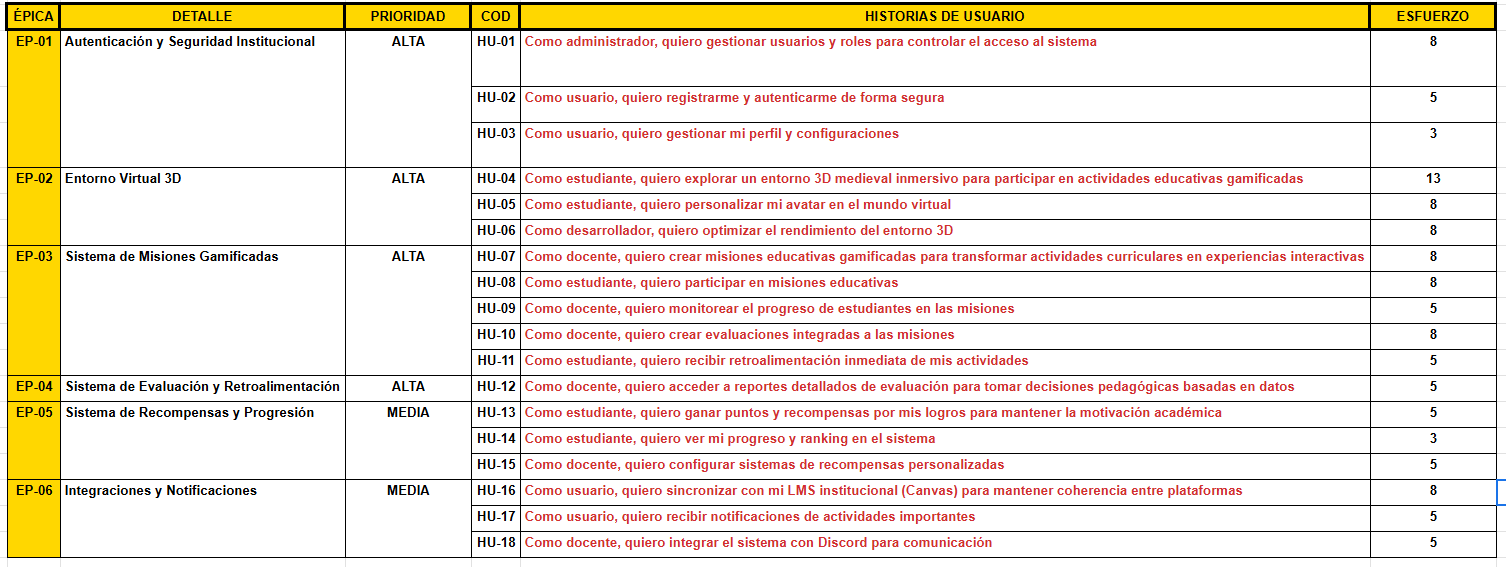
\includegraphics[width=0.85\textwidth]{images/epicas.png}
	\caption{Diagrama de épicas del proyecto.}
	\label{fig:epicas}
\end{figure}

\begin{figure}[H]
	\centering
	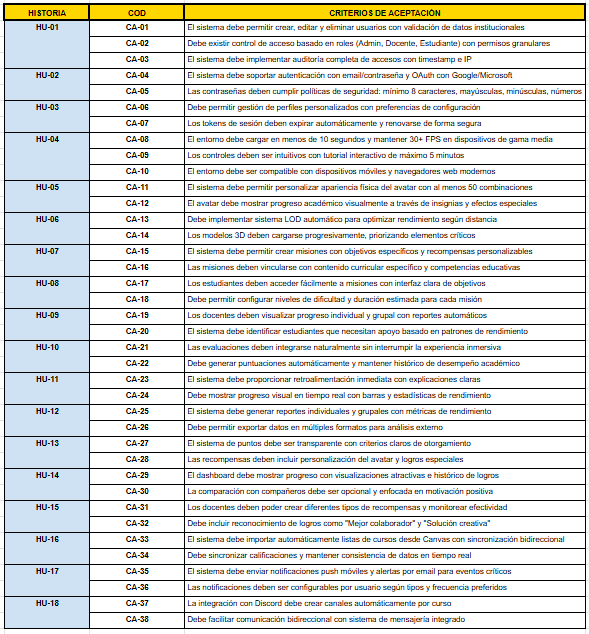
\includegraphics[width=0.85\textwidth]{images/historias_de_usuario.png}
	\caption{Historias de usuario detalladas por épica.}
	\label{fig:historias-usuario}
\end{figure}

\subsubsection{3.2.3 Criterios de aceptación}
Ejemplos de criterios asociados a historias clave:
\begin{itemize}
	\item Autenticación: flujo completo OAuth2 + JWT, expiración configurable, refresco transparente.
	\item Creación de misión: validación de campos obligatorios, guardado atómico, versionado de cambios.
	\item Evaluación automática: registro de puntuación y tiempo, asignación de recompensas según umbrales.
	\item Progreso visual: actualización en tiempo real del nivel tras recibir puntos.
	\item Analítica: métricas mínimas (tiempo activo, misiones completadas, ratio abandono) exportables en CSV.
\end{itemize}

\begin{table}[ht]
	\centering
	\caption{Criterios de aceptación por historia (Tabla 15).}
	\begin{tabular}{p{3.2cm} p{9.8cm}}
		\toprule
		Historia & Criterios (resumen) \\
		\midrule
		Registro & Email institucional verificado, password seguro, confirmación por enlace.\\
		Login & Token válido emitido, revocación en logout, bloqueo tras intentos fallidos.\\
		Crear misión & Objetivos >=1, recompensa asignada, retroalimentación opcional, estado inicial Borrador.\\
		Completar misión & Cambia estado a Completada, asigna puntos y XP, registra timestamp.\\
		Ver progreso & Muestra nivel, XP restante, logros recientes y próximas recompensas.\\
		Panel analítica & Filtra por curso, fecha y tipo de misión; exporta reporte.\\
		Notificación & Envío push dentro de 10s tras publicación de misión.\\
		\bottomrule
	\end{tabular}
\end{table}

\subsection{3.3 Planificación (Gantt)}
El diagrama de Gantt representa la programación de actividades a lo largo del tiempo, mostrando duración, secuencia y dependencias. El proyecto se planifica en 24 semanas distribuidas en seis fases estratégicas.
\begin{itemize}
	\item \textbf{Fase 1 (Sem 1-4) Análisis y Diseño}: requisitos, stakeholders, historias, arquitectura, DER.
		\item \textbf{Fase 2 (Sem 5-10) Backend / API}: implementación de Next.js API routes con TypeScript, autenticación, gestión de usuarios, endpoints para misiones, evaluación automática e integraciones con LMS.
	\item \textbf{Fase 3 (Sem 11-16) Frontend}: interfaz React, entorno 3D, dashboard, app móvil, avatares.
	\item \textbf{Fase 4 (Sem 17-20) Módulos y Analítica}: algoritmos de engagement, detección de anomalías, personalización.
	\item \textbf{Fase 5 (Sem 21-22) Testing}: pruebas integración, seguridad, rendimiento, usabilidad.
	\item \textbf{Fase 6 (Sem 23-24) Despliegue y Capacitación}: infraestructura cloud, CI/CD, formación docente.
\end{itemize}

\begin{figure}[H]
	\centering
	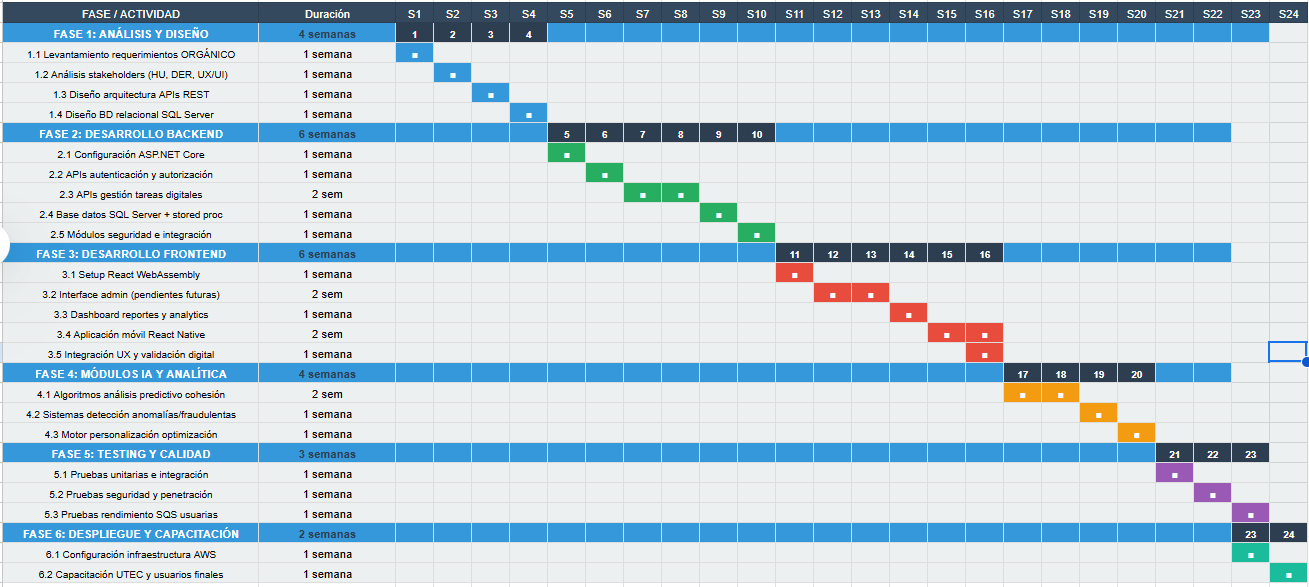
\includegraphics[width=0.95\textwidth]{images/gantt.png}
	\caption{Diagrama de Gantt del proyecto.}
	\label{fig:gantt}
\end{figure}

\section{CAPÍTULO IV: Desarrollo del proyecto}

\subsection{4.1 Metodología de desarrollo}

Para el desarrollo de la plataforma de gamificación educativa se adoptó la metodología Kanban, seleccionada por su flexibilidad para equipos pequeños y su capacidad de adaptación a flujos de trabajo variables. Esta metodología permite gestionar el desarrollo iterativo mediante un tablero visual que facilita el seguimiento del progreso y la identificación de cuellos de botella.

\subsubsection{4.1.1 Configuración del tablero Kanban}

El tablero Kanban se estructuró en las siguientes columnas para optimizar el flujo de trabajo del proyecto:

\begin{itemize}
\item \textbf{Backlog}: Tareas identificadas y priorizadas pendientes de inicio
\item \textbf{En análisis}: Tareas en proceso de definición técnica y diseño
\item \textbf{En desarrollo}: Implementación activa de funcionalidades
\item \textbf{En pruebas}: Validación y testing de componentes desarrollados  
\item \textbf{En revisión}: Revisión de código y documentación
\item \textbf{Finalizado}: Tareas completadas e integradas al sistema
\end{itemize}

\begin{figure}[H]
	\centering
	\fbox{\parbox{0.8\textwidth}{\centering \textbf{Placeholder: Tablero Kanban del Proyecto}\\ \vspace{1cm} Figura mostrando la configuración del tablero Kanban con las columnas definidas y ejemplos de tarjetas de trabajo en diferentes estados del flujo.}}
	\caption{Configuración del tablero Kanban para el desarrollo del proyecto (Figura 14).}
	\label{fig:kanban-board}
\end{figure}

\subsubsection{4.1.2 Límites de trabajo en progreso (WIP)}

Se establecieron límites WIP para mantener la eficiencia del flujo y evitar la sobrecarga de trabajo:

\begin{itemize}
\item \textbf{En análisis}: Máximo 3 elementos
\item \textbf{En desarrollo}: Máximo 4 elementos  
\item \textbf{En pruebas}: Máximo 2 elementos
\item \textbf{En revisión}: Máximo 2 elementos
\end{itemize}

\begin{figure}[H]
	\centering
	\fbox{\parbox{0.8\textwidth}{\centering \textbf{Placeholder: Métricas de Flujo Kanban}\\ \vspace{1cm} Gráfico mostrando el tiempo de ciclo, throughput y distribución del trabajo a lo largo del desarrollo del proyecto.}}
	\caption{Métricas de rendimiento del flujo Kanban durante el desarrollo (Figura 15).}
	\label{fig:kanban-metrics}
\end{figure}

\subsection{4.2 Entregables del proyecto}

El desarrollo se organizó en iteraciones incrementales, con entregables específicos que aportan valor funcional al sistema. Cada entregable fue gestionado a través del tablero Kanban, desde su conceptualización hasta su implementación completa.

\subsubsection{4.2.1 Sprint 0: Configuración inicial}

\paragraph{Entregables}
\begin{itemize}
\item Configuración del entorno de desarrollo (Node.js, PostgreSQL, Docker)
\item Estructura base del proyecto con Next.js y TypeScript
\item Configuración de Prisma ORM y esquema inicial de base de datos
\item Pipeline de CI/CD básico
\end{itemize}

\begin{figure}[H]
	\centering
	\fbox{\parbox{0.8\textwidth}{\centering \textbf{Placeholder: Arquitectura del Entorno de Desarrollo}\\ \vspace{1cm} Diagrama mostrando la configuración del entorno local y cloud, incluyendo bases de datos, servicios y herramientas de desarrollo.}}
	\caption{Configuración del entorno de desarrollo del proyecto (Figura 16).}
	\label{fig:dev-environment}
\end{figure}

\subsubsection{4.2.2 Sprint 1: Sistema de autenticación}

\paragraph{Entregables}
\begin{itemize}
\item Implementación de autenticación JWT con NextAuth.js
\item Integración con proveedores OAuth2 (Google, Microsoft)
\item Sistema de roles y permisos (estudiante, docente, administrador)
\item Interfaces de login y registro de usuarios
\end{itemize}

\begin{figure}[H]
	\centering
	\fbox{\parbox{0.8\textwidth}{\centering \textbf{Placeholder: Flujo de Autenticación}\\ \vspace{1cm} Diagrama de secuencia mostrando el proceso de autenticación desde el login hasta la obtención del token JWT y acceso a recursos protegidos.}}
	\caption{Diagrama de flujo del sistema de autenticación implementado (Figura 17).}
	\label{fig:auth-flow}
\end{figure}

\subsubsection{4.2.3 Sprint 2: Gestión de usuarios y perfiles}

\paragraph{Entregables}
\begin{itemize}
\item CRUD completo para gestión de usuarios
\item Sistema de perfiles con avatares personalizables
\item Dashboard diferenciado por rol de usuario
\item Configuraciones de privacidad y notificaciones
\end{itemize}

\begin{figure}[H]
	\centering
	\fbox{\parbox{0.8\textwidth}{\centering \textbf{Placeholder: Dashboard de Gestión de Usuarios}\\ \vspace{1cm} Captura de pantalla del panel administrativo mostrando la gestión de usuarios, asignación de roles y configuración de perfiles.}}
	\caption{Panel de administración para gestión de usuarios y perfiles (Figura 18).}
	\label{fig:user-management}
\end{figure}

\subsubsection{4.2.4 Sprint 3: Motor de gamificación}

\paragraph{Entregables}
\begin{itemize}
\item Sistema de puntos y niveles
\item Gestión de logros e insignias
\item Algoritmo de progresión basado en actividades
\item API para tracking de eventos de gamificación
\end{itemize}

\begin{figure}[H]
	\centering
	\fbox{\parbox{0.8\textwidth}{\centering \textbf{Placeholder: Arquitectura del Motor de Gamificación}\\ \vspace{1cm} Diagrama de componentes mostrando el motor de gamificación, sistema de puntos, logros y su integración con el sistema académico.}}
	\caption{Arquitectura del motor de gamificación y sistema de progresión (Figura 19).}
	\label{fig:gamification-engine}
\end{figure}

\subsubsection{4.2.5 Sprint 4: Entorno 3D con Three.js}

\paragraph{Entregables}
\begin{itemize}
\item Integración de Three.js en el frontend React
\item Escena 3D básica con mundo medieval
\item Sistema de avatares tridimensionales
\item Controles de navegación e interacción
\end{itemize}

\begin{figure}[H]
	\centering
	\fbox{\parbox{0.8\textwidth}{\centering \textbf{Placeholder: Entorno 3D Medieval}\\ \vspace{1cm} Captura del mundo virtual 3D mostrando el ambiente medieval, avatares de estudiantes y elementos interactivos de gamificación.}}
	\caption{Vista del entorno virtual 3D implementado con Three.js (Figura 20).}
	\label{fig:3d-environment}
\end{figure}

\subsubsection{4.2.6 Sprint 5: Sistema de misiones educativas}

\paragraph{Entregables}
\begin{itemize}
\item Creador de misiones para docentes
\item Sistema de asignación automática y manual
\item Tracking de progreso en tiempo real
\item Integración con el motor de gamificación
\end{itemize}

\begin{figure}[H]
	\centering
	\fbox{\parbox{0.8\textwidth}{\centering \textbf{Placeholder: Creador de Misiones}\\ \vspace{1cm} Interfaz del sistema de creación de misiones mostrando formularios, configuración de objetivos y asignación de recompensas.}}
	\caption{Sistema de creación y gestión de misiones educativas (Figura 21).}
	\label{fig:mission-creator}
\end{figure}

\subsection{4.3 Gestión de riesgos y contingencias}

Durante el desarrollo se implementaron estrategias de mitigación de riesgos basadas en la flexibilidad de Kanban para adaptar el flujo de trabajo ante contingencias.

\subsubsection{4.3.1 Identificación de riesgos técnicos}

\begin{itemize}
\item \textbf{Rendimiento del entorno 3D}: Optimización de mallas y texturas
\item \textbf{Escalabilidad de la base de datos}: Implementación de índices y consultas optimizadas  
\item \textbf{Compatibilidad cross-browser}: Testing en múltiples navegadores
\item \textbf{Seguridad de autenticación}: Implementación de buenas prácticas de seguridad
\end{itemize}

\begin{figure}[H]
	\centering
	\fbox{\parbox{0.8\textwidth}{\centering \textbf{Placeholder: Matriz de Riesgos del Proyecto}\\ \vspace{1cm} Matriz mostrando la identificación, probabilidad, impacto y estrategias de mitigación de los principales riesgos técnicos del proyecto.}}
	\caption{Matriz de análisis de riesgos y estrategias de mitigación (Figura 22).}
	\label{fig:risk-matrix}
\end{figure}

\subsection{4.4 Control de versiones y colaboración}

Se estableció un flujo de trabajo con Git que facilita la colaboración y el control de versiones del código fuente.

\subsubsection{4.4.1 Estrategia de branching}

\begin{itemize}
\item \textbf{main}: Rama principal con código estable en producción
\item \textbf{develop}: Rama de desarrollo con últimas características integradas
\item \textbf{feature/*}: Ramas para desarrollo de funcionalidades específicas
\item \textbf{hotfix/*}: Ramas para correcciones críticas en producción
\end{itemize}

\begin{figure}[H]
	\centering
	\fbox{\parbox{0.8\textwidth}{\centering \textbf{Placeholder: Flujo de Git Branching}\\ \vspace{1cm} Diagrama mostrando la estrategia de ramificación Git utilizada, con ejemplos de merge requests y flujo de integración continua.}}
	\caption{Estrategia de branching y flujo de trabajo con Git (Figura 23).}
	\label{fig:git-workflow}
\end{figure}

\section{CAPÍTULO V: Producto final}

Este capítulo presenta la documentación completa del producto final, incluyendo los manuales necesarios para que usuarios finales y personal técnico puedan utilizar, operar y mantener la plataforma educativa 3D de gamificación de tareas académicas. Se incluyen dos manuales fundamentales: el Manual del Usuario, orientado a estudiantes, docentes y administradores que interactuarán con la plataforma; y el Manual del Sistema, dirigido al personal técnico encargado de la instalación, configuración, mantenimiento y resolución de problemas del sistema.

\subsection{5.1 Manual de usuario}

El Manual del Usuario proporciona instrucciones detalladas sobre el uso de la plataforma desde la perspectiva de los tres roles principales: estudiantes, docentes y administradores. Cada sección incluye guías paso a paso, capturas de pantalla y buenas prácticas para maximizar el valor educativo de la aplicación.

\subsubsection{5.1.1 Introducción a la plataforma}

La plataforma Warclass es una aplicación educativa 3D que transforma las tareas académicas tradicionales en experiencias de aprendizaje inmersivas mediante la gamificación. El sistema permite a los docentes crear misiones educativas que los estudiantes completan en un entorno virtual medieval, ganando puntos, subiendo de nivel y desbloqueando logros mientras aprenden.

\paragraph{Acceso a la plataforma}

La plataforma está disponible en versión web y móvil:

\begin{itemize}
	\item \textbf{Versión Web}: Accesible desde cualquier navegador moderno (Chrome, Firefox, Safari, Edge) en la URL proporcionada por su institución educativa.
	\item \textbf{Versión Móvil}: Aplicación nativa disponible para Android e iOS, descargable desde las tiendas oficiales.
\end{itemize}

\paragraph{Requisitos del sistema}

\begin{table}[H]
	\centering
	\caption{Requisitos mínimos del sistema para usuarios.}
	\begin{tabular}{p{4cm} p{9cm}}
		\toprule
		Componente & Requisitos \\
		\midrule
		Navegador Web & Chrome 90+, Firefox 88+, Safari 14+, Edge 90+ \\
		Conexión Internet & Mínimo 5 Mbps (10 Mbps recomendado) \\
		Resolución & 1366x768 mínimo (1920x1080 recomendado) \\
		Hardware & CPU: Dual Core 2.0 GHz, RAM: 4GB, GPU: Compatible WebGL 2.0 \\
		Sistema Operativo Móvil & Android 9.0+ o iOS 13.0+ \\
		\bottomrule
	\end{tabular}
\end{table}

\subsubsection{5.1.2 Registro y autenticación}

\paragraph{Crear una cuenta}

Los usuarios pueden registrarse utilizando su correo institucional o mediante autenticación OAuth2 con proveedores autorizados (Google Workspace, Microsoft 365).

\textbf{Proceso de registro con correo institucional:}

\begin{enumerate}
	\item Acceder a la URL de la plataforma proporcionada por su institución
	\item Hacer clic en el botón ``Registrarse''
	\item Ingresar correo electrónico institucional
	\item Crear una contraseña segura (mínimo 8 caracteres, incluyendo mayúsculas, minúsculas, números y símbolos)
	\item Completar datos del perfil: nombre completo, código de estudiante/docente, institución
	\item Aceptar los términos de servicio y políticas de privacidad
	\item Verificar el correo electrónico mediante el enlace enviado
	\item Iniciar sesión con las credenciales creadas
\end{enumerate}

\begin{figure}[H]
	\centering
	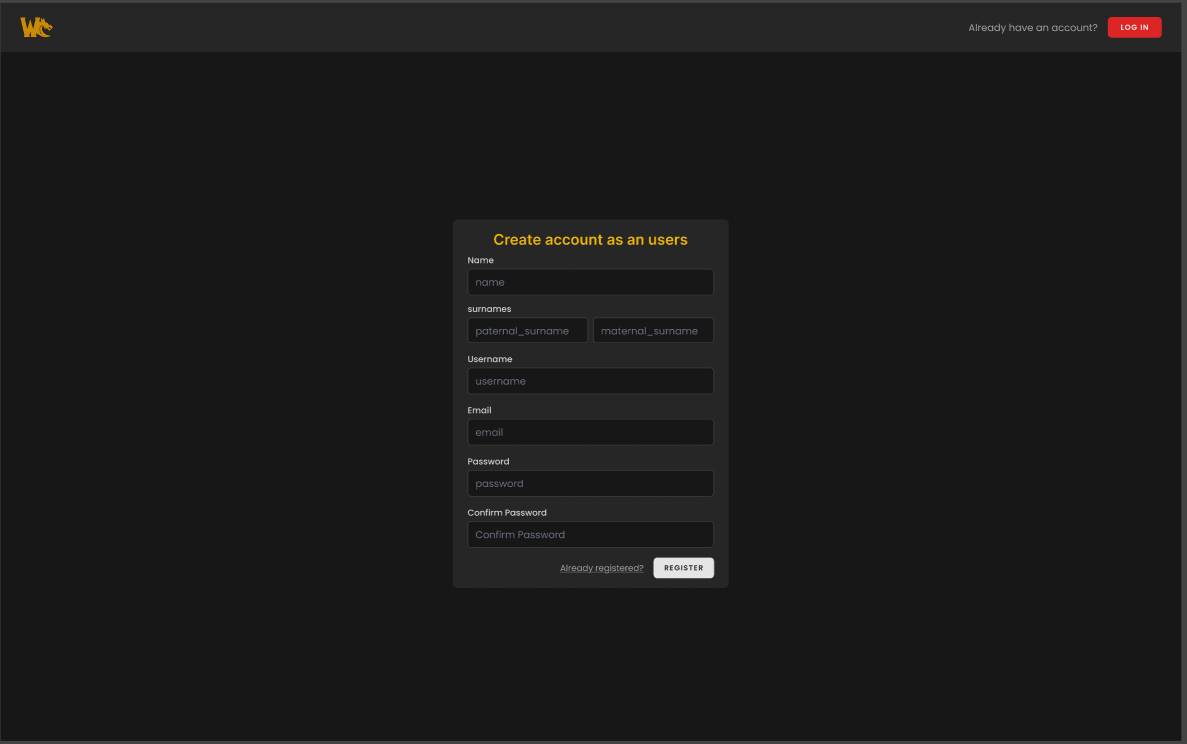
\includegraphics[width=0.75\textwidth]{images/pagina_web_registro.png}
	\caption{Pantalla de registro de usuario con formulario de datos básicos.}
	\label{fig:manual-registro}
\end{figure}

\textbf{Proceso de registro con OAuth2:}

\begin{enumerate}
	\item Hacer clic en ``Iniciar sesión con Google'' o ``Iniciar sesión con Microsoft''
	\item Autorizar el acceso a su cuenta institucional
	\item Completar datos adicionales si es necesario
	\item Confirmar creación de cuenta
\end{enumerate}

\begin{figure}[H]
	\centering
	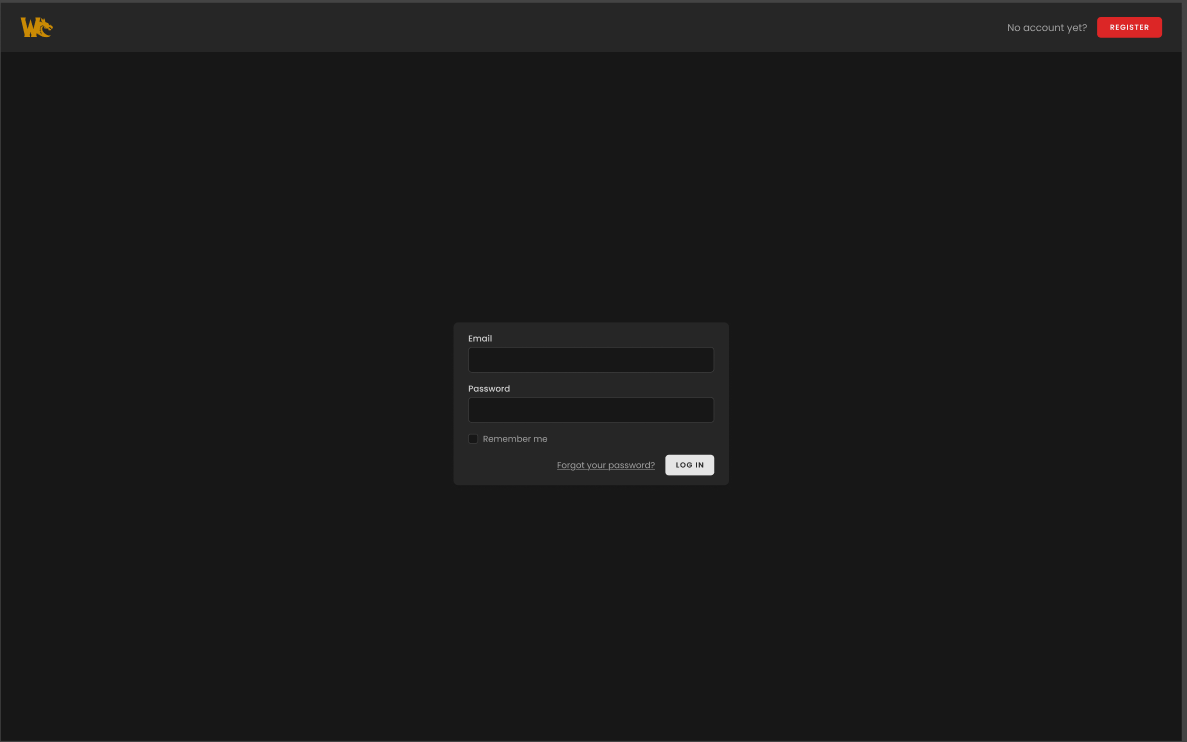
\includegraphics[width=0.75\textwidth]{images/pagina_web_iniciar-sesion.png}
	\caption{Pantalla de inicio de sesión con opciones de autenticación.}
	\label{fig:manual-login}
\end{figure}

\paragraph{Inicio de sesión}

\begin{enumerate}
	\item Ingresar correo electrónico y contraseña
	\item (Opcional) Marcar ``Recordarme'' para mantener la sesión activa
	\item Hacer clic en ``Iniciar sesión''
	\item Si olvidó su contraseña, usar la opción ``¿Olvidaste tu contraseña?''
\end{enumerate}

\paragraph{Recuperación de contraseña}

\begin{enumerate}
	\item Hacer clic en ``¿Olvidaste tu contraseña?''
	\item Ingresar correo electrónico registrado
	\item Revisar bandeja de entrada y seguir las instrucciones del correo
	\item Crear nueva contraseña segura
	\item Iniciar sesión con la nueva contraseña
\end{enumerate}

\subsubsection{5.1.3 Manual para estudiantes}

\paragraph{Dashboard del estudiante}

Al iniciar sesión, el estudiante accede a su dashboard personalizado que muestra:

\begin{itemize}
	\item \textbf{Vista del avatar 3D}: Representación visual del progreso y equipamiento actual
	\item \textbf{Nivel y experiencia (XP)}: Barra de progreso que muestra el nivel actual y experiencia necesaria para el siguiente nivel
	\item \textbf{Misiones activas}: Lista de tareas académicas disponibles y en progreso
	\item \textbf{Notificaciones}: Alertas de nuevas misiones, logros desbloqueados y mensajes de docentes
	\item \textbf{Logros recientes}: Insignias y reconocimientos obtenidos
	\item \textbf{Estadísticas}: Tiempo de estudio, misiones completadas, puntos ganados
\end{itemize}

\paragraph{Personalización del avatar}

El avatar 3D es la representación visual del estudiante en el entorno virtual. Su apariencia evoluciona con el progreso académico.

\textbf{Pasos para personalizar el avatar:}

\begin{enumerate}
	\item Hacer clic en el avatar en el dashboard
	\item Seleccionar la pestaña ``Personalizar''
	\item Elegir características disponibles según el nivel:
	\begin{itemize}
		\item \textbf{Género}: Masculino, Femenino, Otro
		\item \textbf{Tono de piel}: Paleta de colores disponible
		\item \textbf{Cabello}: Estilo y color (se desbloquean con niveles)
		\item \textbf{Ojos}: Color y forma
		\item \textbf{Ropa}: Atuendos medievales desbloqueables
		\item \textbf{Accesorios}: Armas decorativas, escudos, capas (requieren logros)
	\end{itemize}
	\item Previsualizar cambios en tiempo real en el visor 3D
	\item Hacer clic en ``Guardar cambios''
\end{enumerate}

\paragraph{Explorar y aceptar misiones}

Las misiones son las actividades académicas gamificadas creadas por los docentes.

\textbf{Tipos de misiones:}

\begin{itemize}
	\item \textbf{Misión Principal}: Actividad obligatoria vinculada al currículo
	\item \textbf{Misión Secundaria}: Actividad opcional para refuerzo o profundización
	\item \textbf{Misión de Grupo}: Actividad colaborativa con otros estudiantes
	\item \textbf{Desafío}: Competencia temporal con recompensas especiales
\end{itemize}

\textbf{Aceptar una misión:}

\begin{enumerate}
	\item Navegar a la sección ``Misiones Disponibles''
	\item Hacer clic en una misión para ver los detalles:
	\begin{itemize}
		\item Descripción y objetivos de aprendizaje
		\item Dificultad (Novato, Aprendiz, Experto, Maestro)
		\item Recompensas (XP, puntos, ítems)
		\item Fecha límite
		\item Materiales de apoyo
	\end{itemize}
	\item Hacer clic en ``Aceptar Misión''
	\item La misión aparecerá en ``Mis Misiones Activas''
\end{enumerate}

\paragraph{Completar misiones}

\textbf{Desarrollo de la misión:}

\begin{enumerate}
	\item Acceder a la misión desde ``Mis Misiones Activas''
	\item Leer las instrucciones y objetivos específicos
	\item Acceder a materiales de apoyo (videos, documentos, enlaces)
	\item Completar las actividades requeridas:
	\begin{itemize}
		\item Responder cuestionarios interactivos
		\item Subir archivos de trabajo (documentos, imágenes, videos)
		\item Participar en debates en el foro de la misión
		\item Realizar investigaciones y análisis
	\end{itemize}
	\item Usar el chatbot de ayuda si tiene dudas
	\item Guardar progreso automático (la plataforma guarda cada 30 segundos)
	\item Cuando termine, hacer clic en ``Enviar Misión''
\end{enumerate}

\textbf{Evaluación y retroalimentación:}

\begin{enumerate}
	\item El sistema evalúa automáticamente componentes objetivos (cuestionarios, ejercicios)
	\item El docente revisa componentes subjetivos (ensayos, proyectos)
	\item Recibe notificación cuando la misión sea evaluada
	\item Puede ver:
	\begin{itemize}
		\item Calificación obtenida
		\item Comentarios del docente
		\item Áreas de mejora
		\item Respuestas correctas e incorrectas
	\end{itemize}
	\item Si es posible, puede reenviar la misión para mejorar la calificación
\end{enumerate}

\paragraph{Sistema de progresión}

\textbf{Niveles y experiencia (XP):}

\begin{itemize}
	\item Cada misión completada otorga XP según su dificultad
	\item Al acumular suficiente XP, el estudiante sube de nivel
	\item Cada nivel desbloquea nuevas personalizaciones para el avatar
	\item Los niveles se muestran como rangos medievales: Paje (1-5), Escudero (6-10), Caballero (11-20), Paladín (21-30), Leyenda (31+)
\end{itemize}

\textbf{Sistema de puntos:}

\begin{itemize}
	\item Puntos de Conocimiento: Reflejan el dominio académico
	\item Puntos de Participación: Recompensan el engagement
	\item Puntos de Colaboración: Otorgados en misiones grupales
\end{itemize}

\textbf{Logros e insignias:}

\begin{itemize}
	\item \textbf{Logros de dominio}: Por completar conjuntos de misiones relacionadas
	\item \textbf{Logros de velocidad}: Por completar misiones antes del plazo
	\item \textbf{Logros de excelencia}: Por obtener calificaciones perfectas
	\item \textbf{Logros sociales}: Por colaborar efectivamente
	\item \textbf{Logros especiales}: Eventos temporales y desafíos únicos
\end{itemize}

\paragraph{Tabla de clasificación}

La tabla muestra el ranking de estudiantes según diversos criterios:

\begin{itemize}
	\item Ranking general por XP total
	\item Ranking por curso específico
	\item Ranking semanal/mensual
	\item Comparación con compañeros de grupo
\end{itemize}

\textbf{Nota sobre privacidad:} Los estudiantes pueden optar por aparecer de forma anónima en las tablas públicas.

\subsubsection{5.1.4 Manual para docentes}

\paragraph{Dashboard del docente}

El panel de control del docente proporciona una vista integral de todas sus actividades educativas:

\begin{itemize}
	\item \textbf{Resumen de cursos}: Lista de cursos activos con métricas rápidas
	\item \textbf{Misiones pendientes de evaluación}: Trabajos esperando revisión
	\item \textbf{Estadísticas de engagement}: Participación estudiantil en tiempo real
	\item \textbf{Alertas}: Estudiantes con bajo rendimiento o inactividad
	\item \textbf{Analítica}: Gráficos de progreso del grupo
\end{itemize}

\begin{figure}[H]
	\centering
	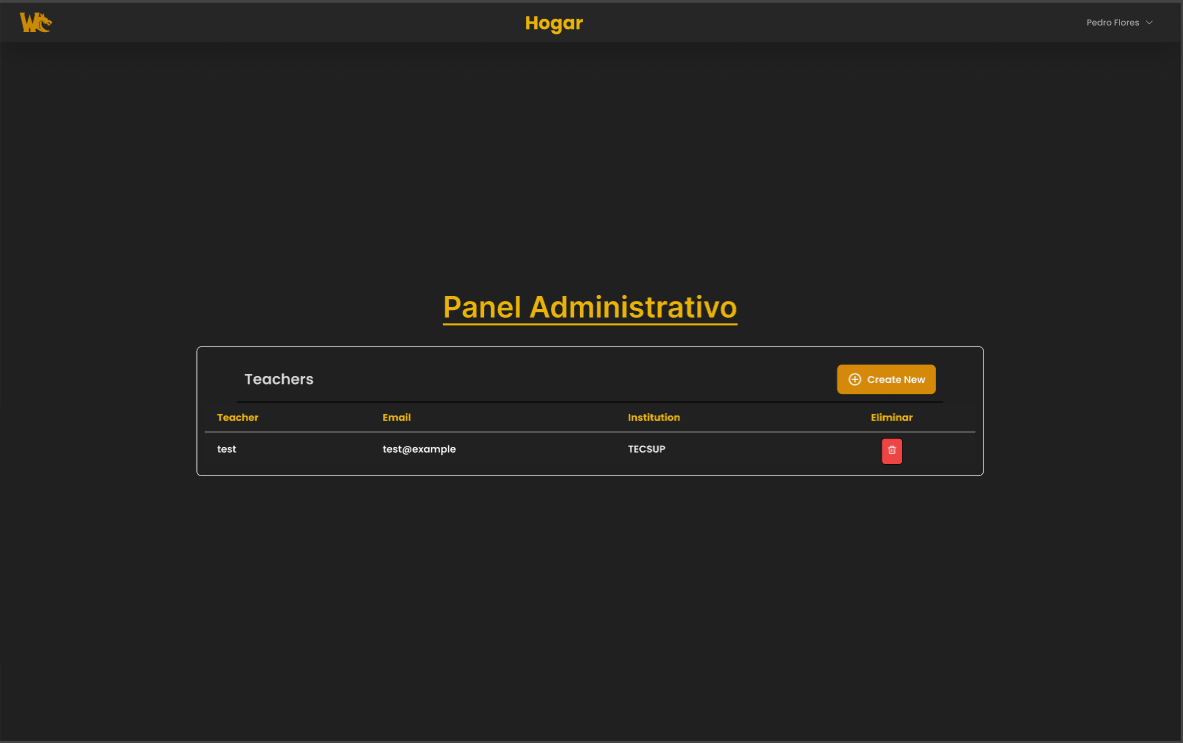
\includegraphics[width=0.75\textwidth]{images/pagina_web_panel-administrativo.png}
	\caption{Panel de administración del docente con vista de cursos y misiones activas.}
	\label{fig:manual-profesor}
\end{figure}

\paragraph{Gestión de cursos}

\textbf{Crear un nuevo curso:}

\begin{enumerate}
	\item Ir a ``Mis Cursos'' > ``Crear Nuevo Curso''
	\item Completar información básica:
	\begin{itemize}
		\item Nombre del curso
		\item Código de curso
		\item Descripción y objetivos de aprendizaje
		\item Período académico
		\item Horario y modalidad
	\end{itemize}
	\item Configurar ajustes de gamificación:
	\begin{itemize}
		\item Esquema de puntos (XP por dificultad)
		\item Niveles y rangos personalizados
		\item Logros específicos del curso
	\end{itemize}
	\item Establecer políticas:
	\begin{itemize}
		\item Política de entregas tardías
		\item Número de reenvíos permitidos
		\item Criterios de evaluación
	\end{itemize}
	\item Hacer clic en ``Crear Curso''
\end{enumerate}

\begin{figure}[H]
	\centering
	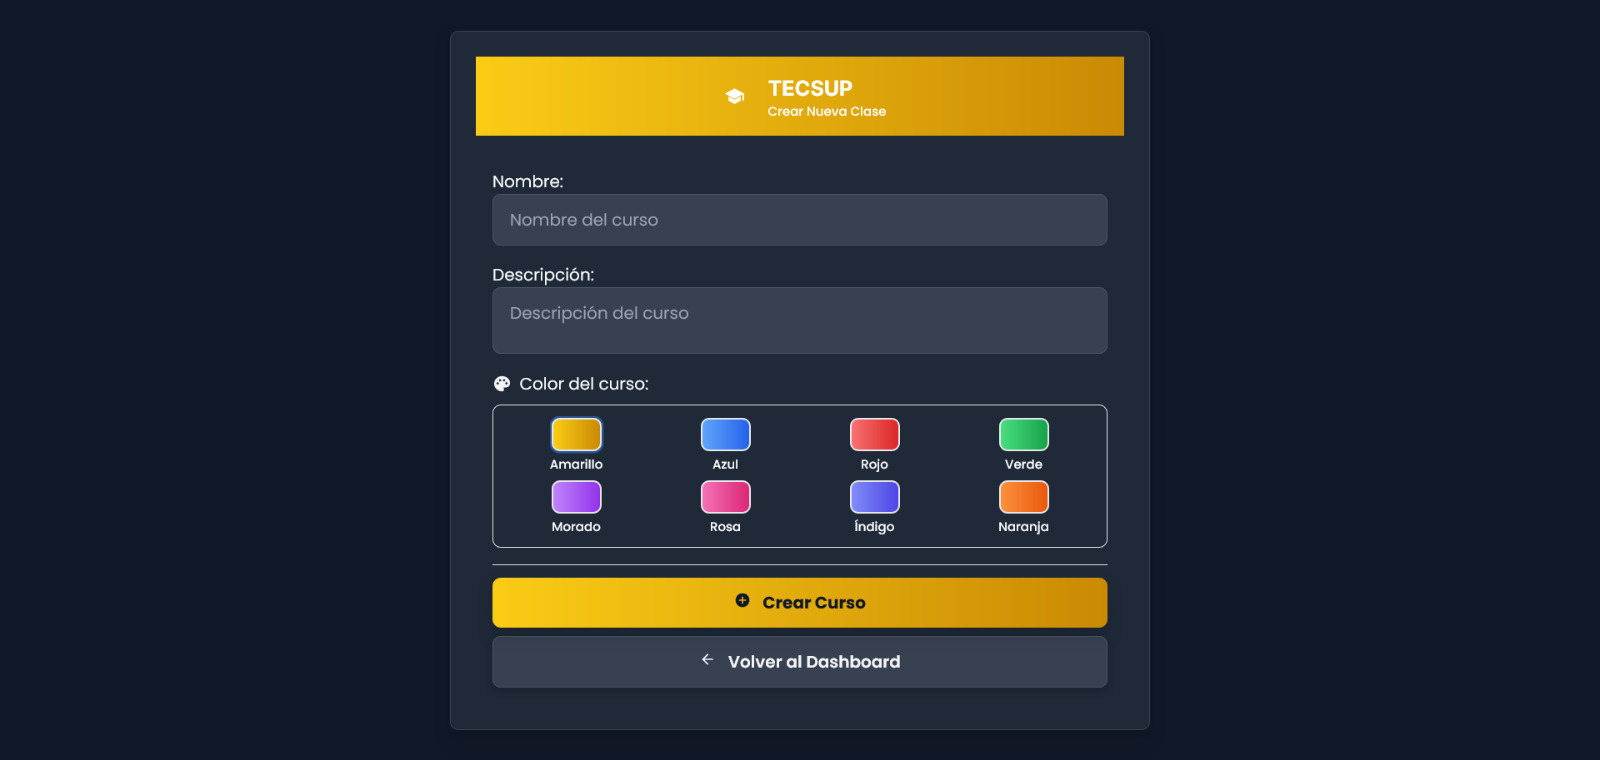
\includegraphics[width=0.75\textwidth]{images/pagina_web_crear-una-clase.jpg}
	\caption{Interfaz para crear un nuevo curso con configuración básica.}
	\label{fig:manual-crear-curso}
\end{figure}

\begin{figure}[H]
	\centering
	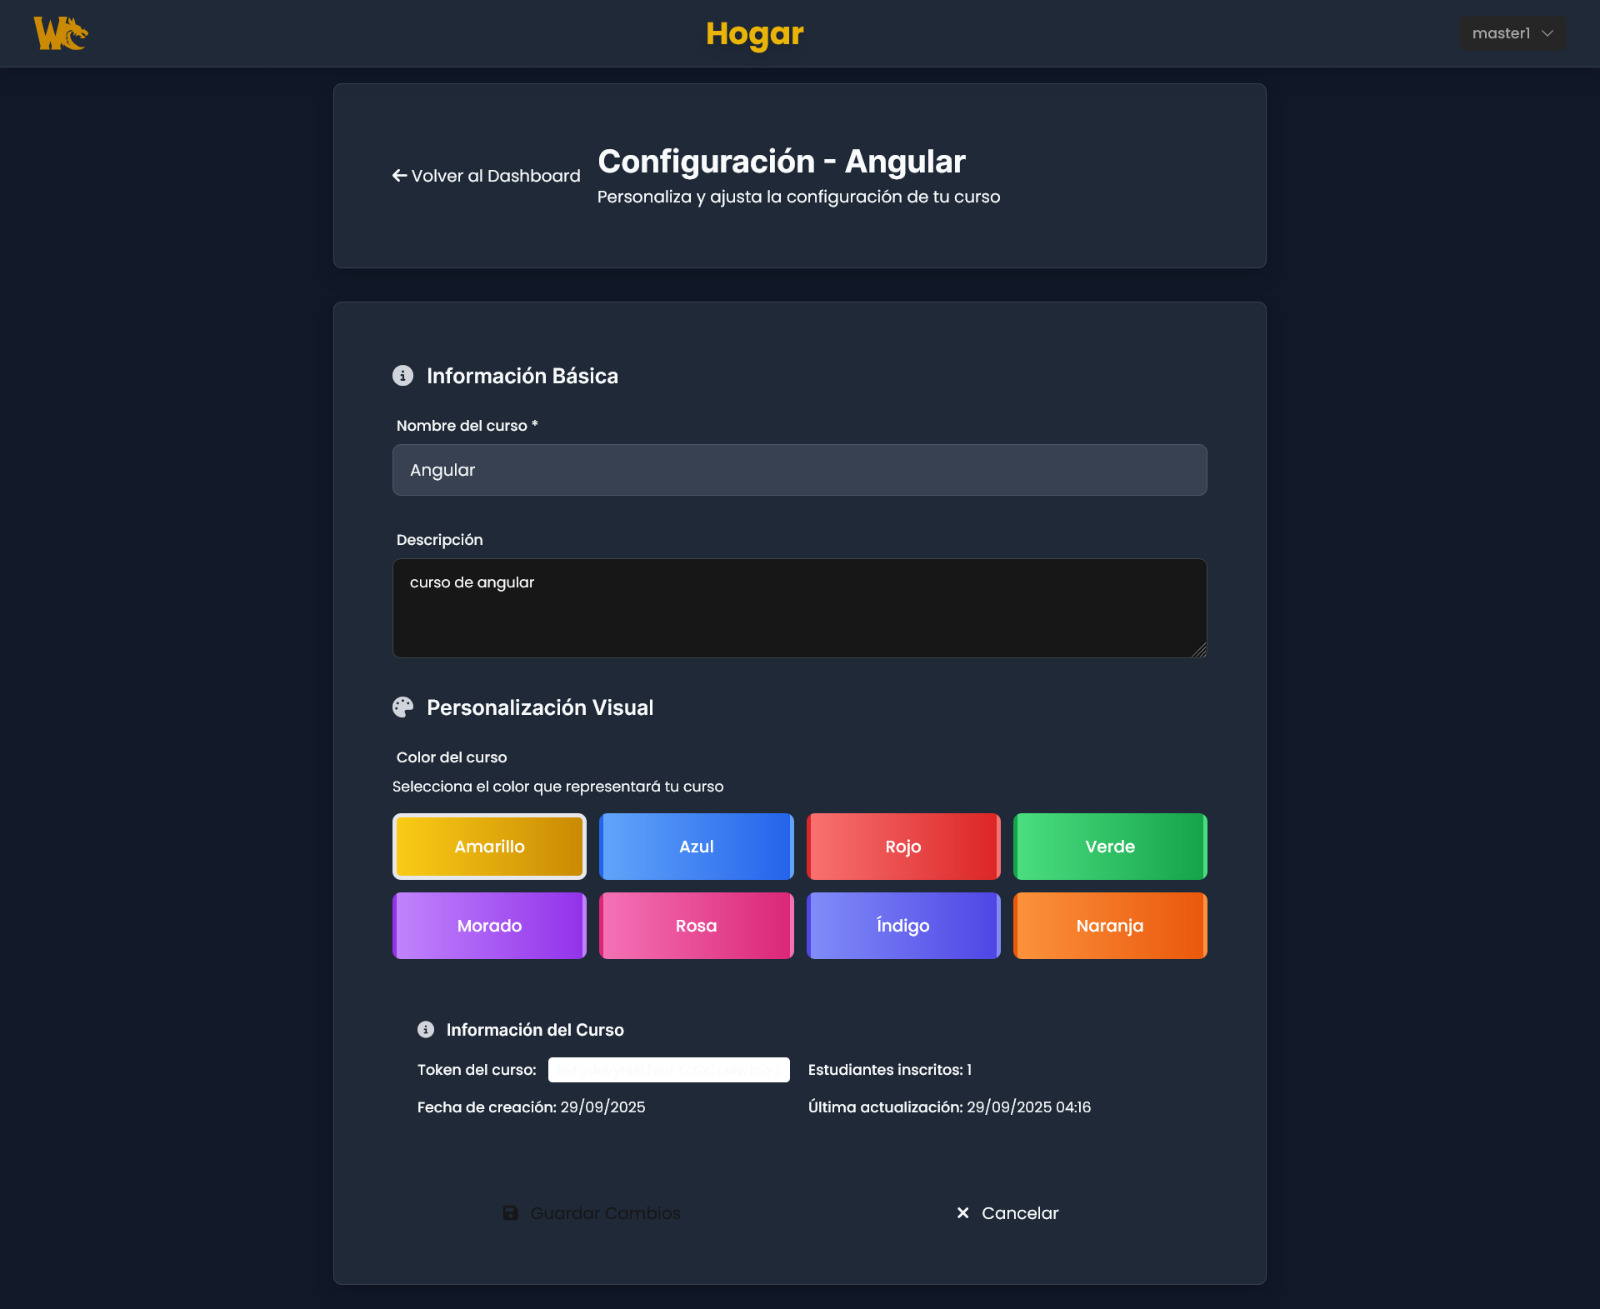
\includegraphics[width=0.75\textwidth]{images/pagina_web_configuracion-de-la.clase.jpg}
	\caption{Configuración de ajustes de gamificación y políticas del curso.}
	\label{fig:manual-config-curso}
\end{figure}

\begin{figure}[H]
	\centering
	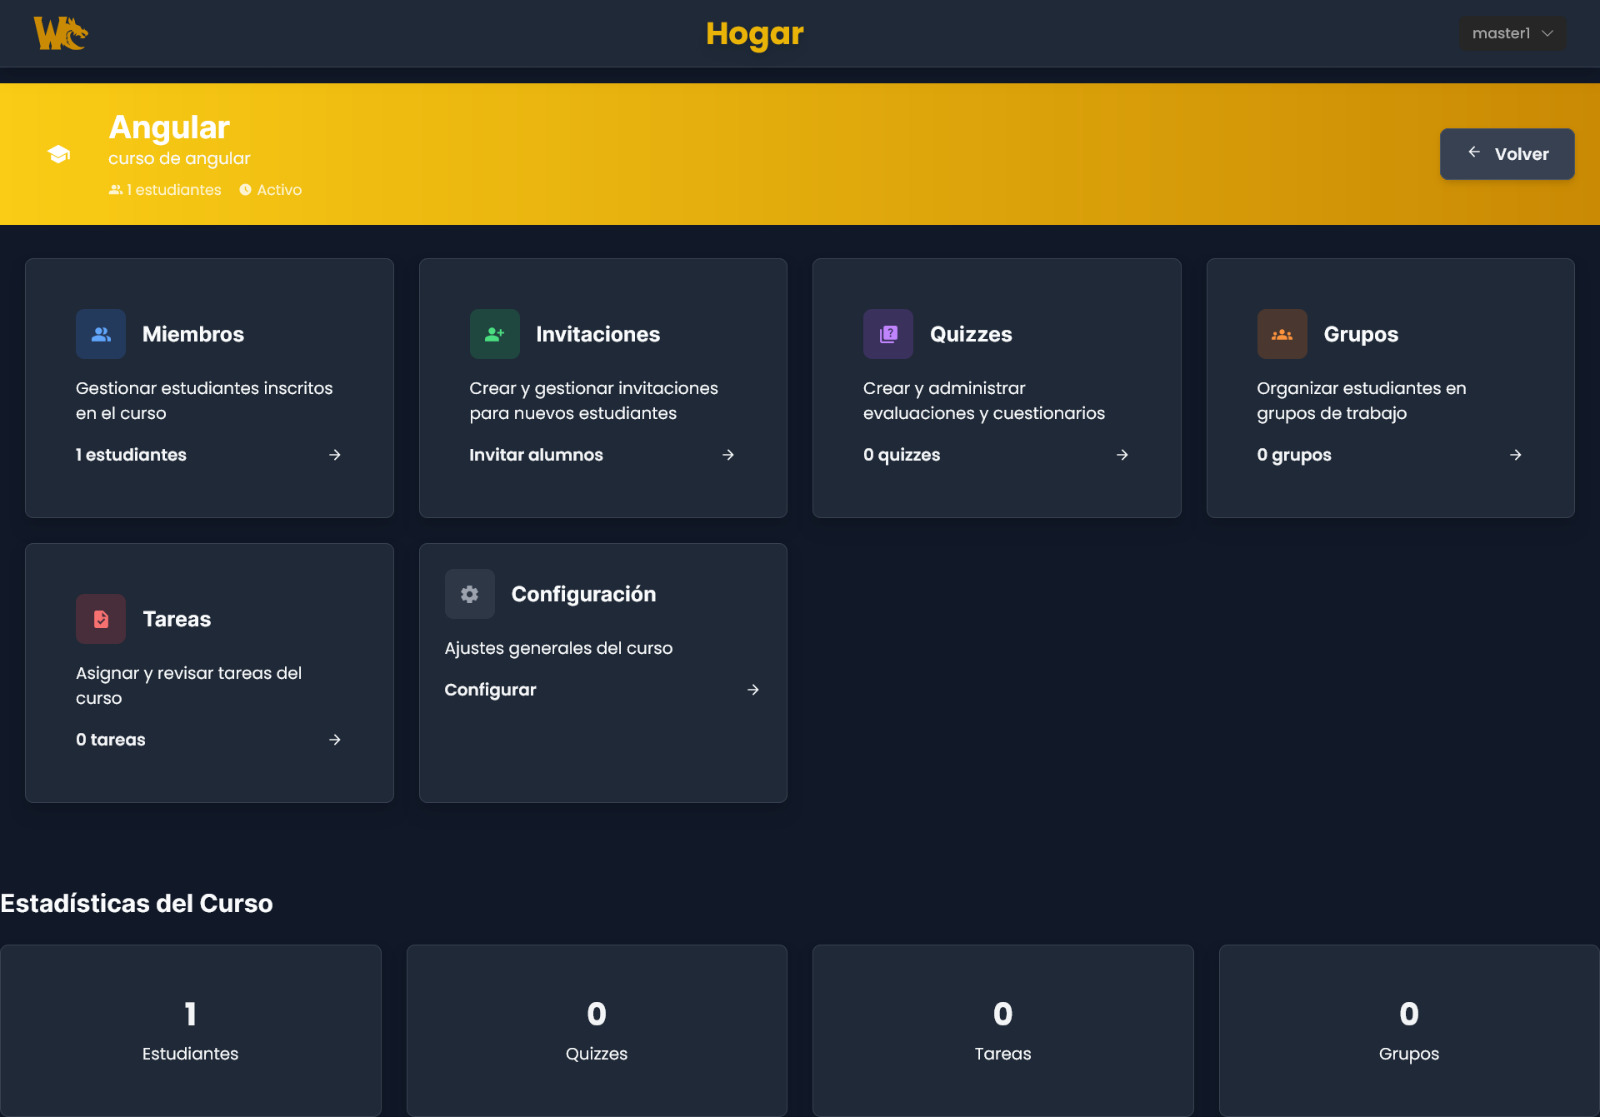
\includegraphics[width=0.75\textwidth]{images/pagina_web_vista-profesor-clase.jpg}
	\caption{Vista principal del profesor para gestión del curso.}
	\label{fig:manual-vista-profesor}
\end{figure}

\textbf{Gestionar estudiantes:}

\begin{enumerate}
	\item Acceder al curso > ``Estudiantes''
	\item Opciones disponibles:
	\begin{itemize}
		\item \textbf{Agregar estudiantes}: Mediante código de curso, lista de correos o integración con Canvas
		\item \textbf{Organizar grupos}: Crear equipos para misiones colaborativas
		\item \textbf{Ver perfiles}: Revisar progreso individual, historial y logros
		\item \textbf{Enviar mensajes}: Comunicación directa o masiva
		\item \textbf{Gestionar permisos}: Roles especiales (moderador de foro, tutor par)
	\end{itemize}
\end{enumerate}

\begin{figure}[H]
	\centering
	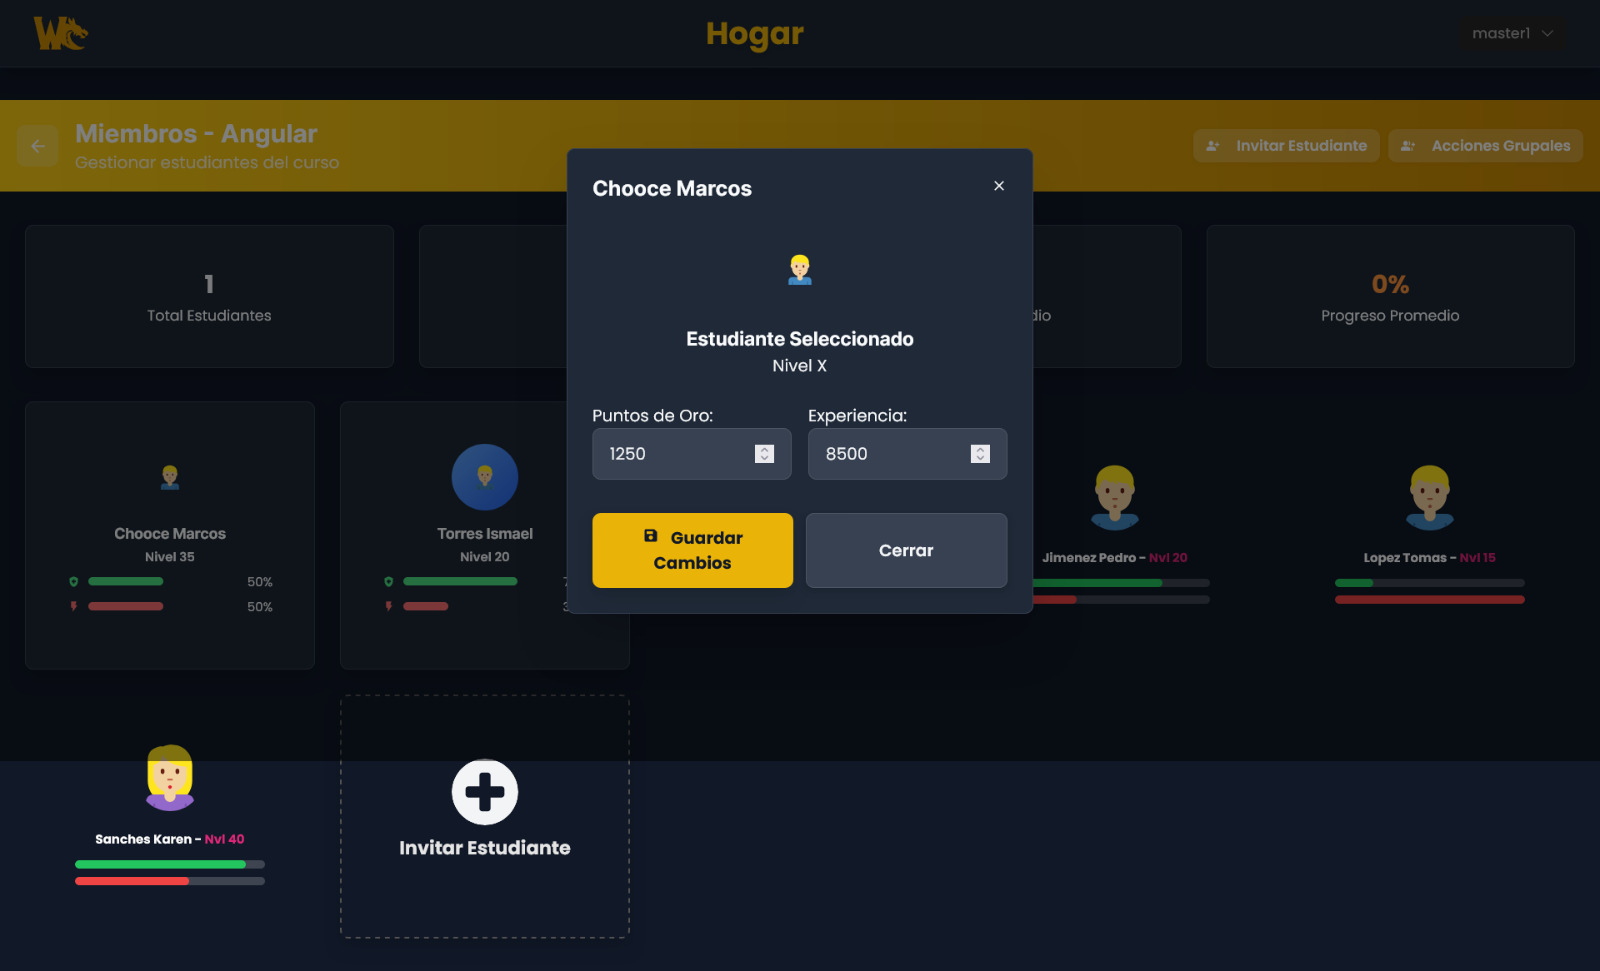
\includegraphics[width=0.75\textwidth]{images/pagina_web_gestionar-alumnos.jpg}
	\caption{Interfaz de gestión de estudiantes con opciones de organización y permisos.}
	\label{fig:manual-gestionar-alumnos}
\end{figure}

\begin{figure}[H]
	\centering
	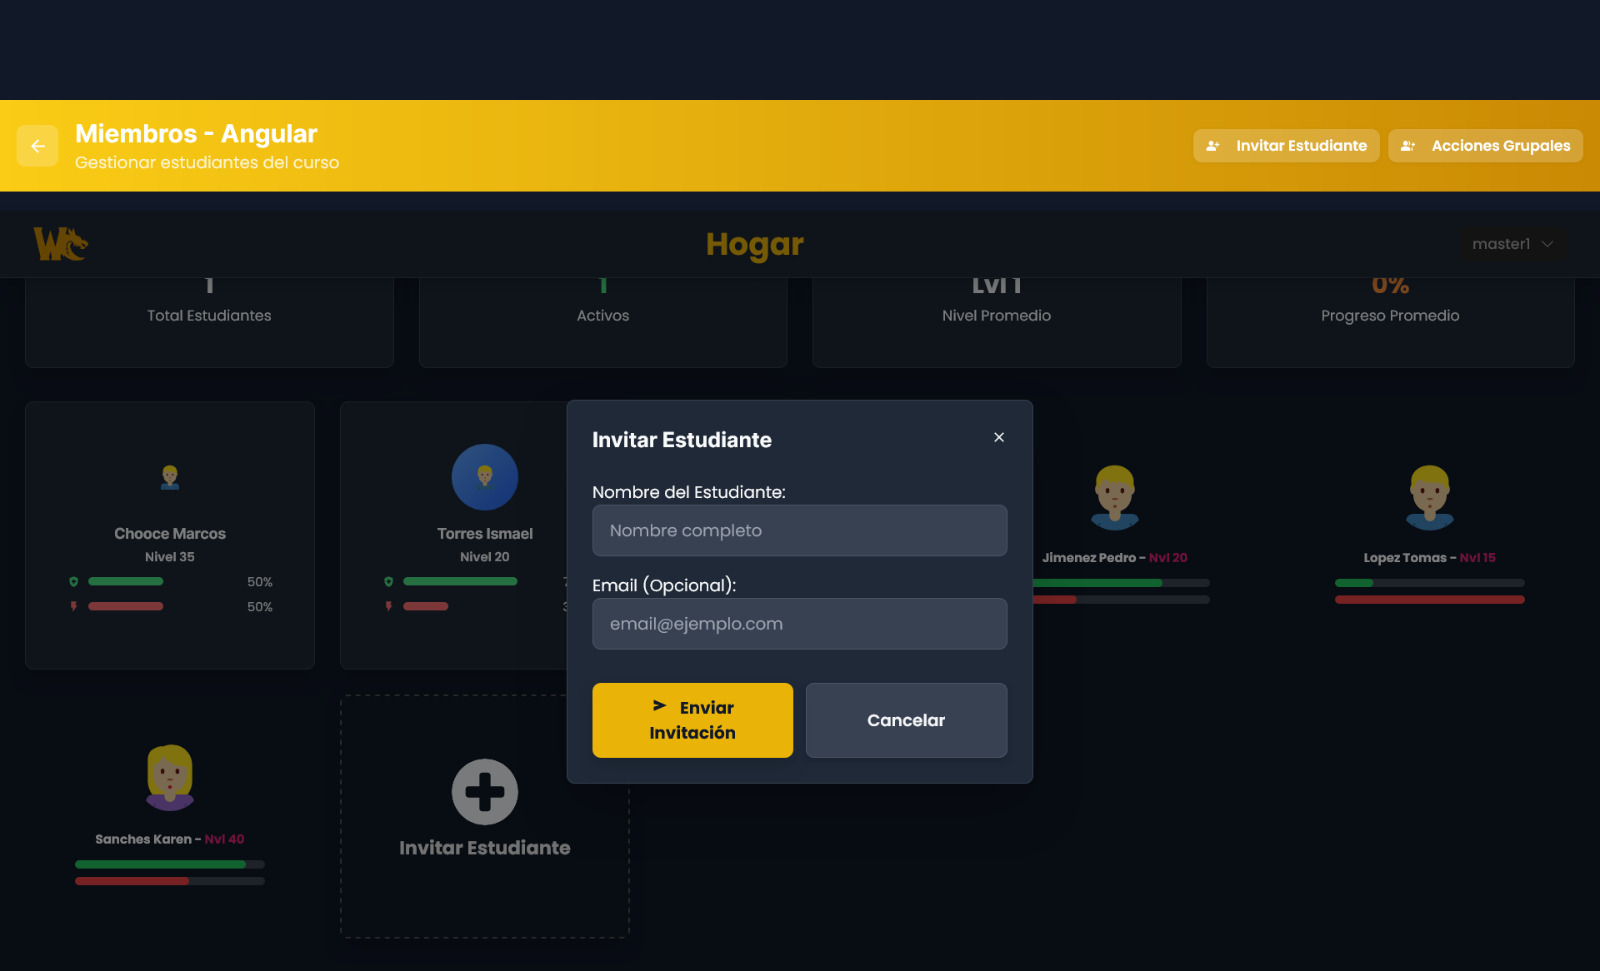
\includegraphics[width=0.75\textwidth]{images/pagina_web_invitar-a-clase.jpg}
	\caption{Sistema de invitación de estudiantes mediante código o correo electrónico.}
	\label{fig:manual-invitar-clase}
\end{figure}

\begin{figure}[H]
	\centering
	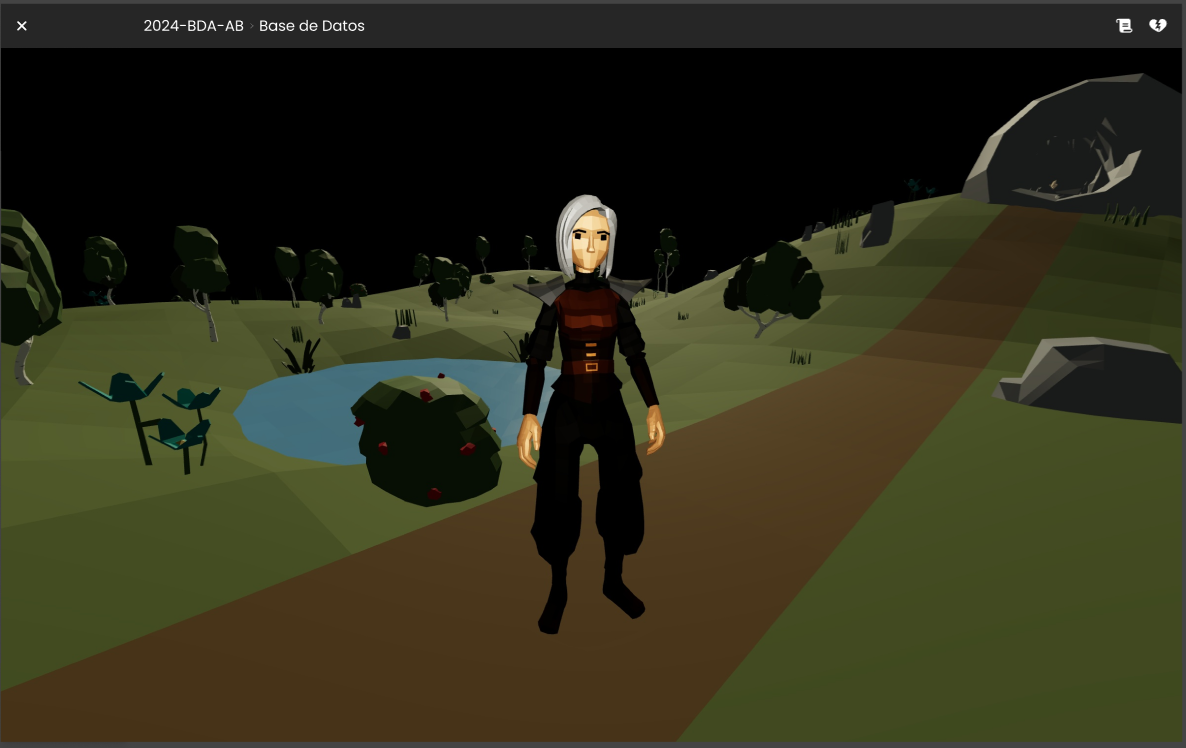
\includegraphics[width=0.75\textwidth]{images/pagina_web_vista-alumno.png}
	\caption{Vista del estudiante mostrando su avatar y progreso en el sistema.}
	\label{fig:manual-vista-alumno}
\end{figure}

\paragraph{Crear misiones educativas}

El creador de misiones permite transformar cualquier actividad académica en una experiencia gamificada.

\textbf{Proceso de creación:}

\begin{enumerate}
	\item Acceder al curso > ``Crear Nueva Misión''
	\item \textbf{Paso 1 - Información básica}:
	\begin{itemize}
		\item Título de la misión (debe ser atractivo)
		\item Descripción narrativa (contextualizar en el mundo medieval)
		\item Tipo de misión (Principal, Secundaria, Grupal, Desafío)
		\item Curso y tema asociado
	\end{itemize}
	\item \textbf{Paso 2 - Objetivos de aprendizaje}:
	\begin{itemize}
		\item Definir competencias a desarrollar
		\item Indicadores de logro
		\item Nivel de dificultad (Novato, Aprendiz, Experto, Maestro)
	\end{itemize}
	\item \textbf{Paso 3 - Contenido y actividades}:
	\begin{itemize}
		\item Agregar instrucciones detalladas
		\item Subir materiales de apoyo (PDF, videos, enlaces)
		\item Configurar actividades:
		\begin{itemize}
			\item Cuestionarios (opción múltiple, verdadero/falso, respuesta corta)
			\item Tareas de entrega (documentos, imágenes, videos)
			\item Foros de discusión
			\item Ejercicios interactivos
		\end{itemize}
	\end{itemize}
	\item \textbf{Paso 4 - Evaluación}:
	\begin{itemize}
		\item Definir criterios de evaluación (rúbricas)
		\item Asignar puntos a cada componente
		\item Configurar evaluación automática para elementos objetivos
		\item Establecer peso de componentes subjetivos
	\end{itemize}
	\item \textbf{Paso 5 - Gamificación}:
	\begin{itemize}
		\item Asignar XP según dificultad
		\item Definir recompensas (ítems virtuales, insignias)
		\item Configurar bonificaciones (por velocidad, calidad)
		\item Agregar logros especiales
	\end{itemize}
	\item \textbf{Paso 6 - Configuración temporal}:
	\begin{itemize}
		\item Fecha de publicación
		\item Fecha límite de entrega
		\item Permitir entregas tardías (con penalización)
		\item Número de intentos permitidos
	\end{itemize}
	\item Previsualizar la misión
	\item Publicar o guardar como borrador
\end{enumerate}

\paragraph{Evaluar trabajos de estudiantes}

\textbf{Proceso de evaluación:}

\begin{enumerate}
	\item Acceder a ``Misiones Pendientes de Evaluación''
	\item Seleccionar una misión para ver las entregas
	\item Para cada estudiante:
	\begin{itemize}
		\item Revisar el trabajo entregado
		\item Ver evaluación automática (si aplica)
		\item Aplicar rúbrica de evaluación
		\item Asignar calificación numérica
		\item Escribir retroalimentación constructiva
		\item Identificar fortalezas y áreas de mejora
		\item Permitir reenvío (opcional)
	\end{itemize}
	\item Guardar evaluación y notificar al estudiante
\end{enumerate}

\begin{figure}[H]
	\centering
	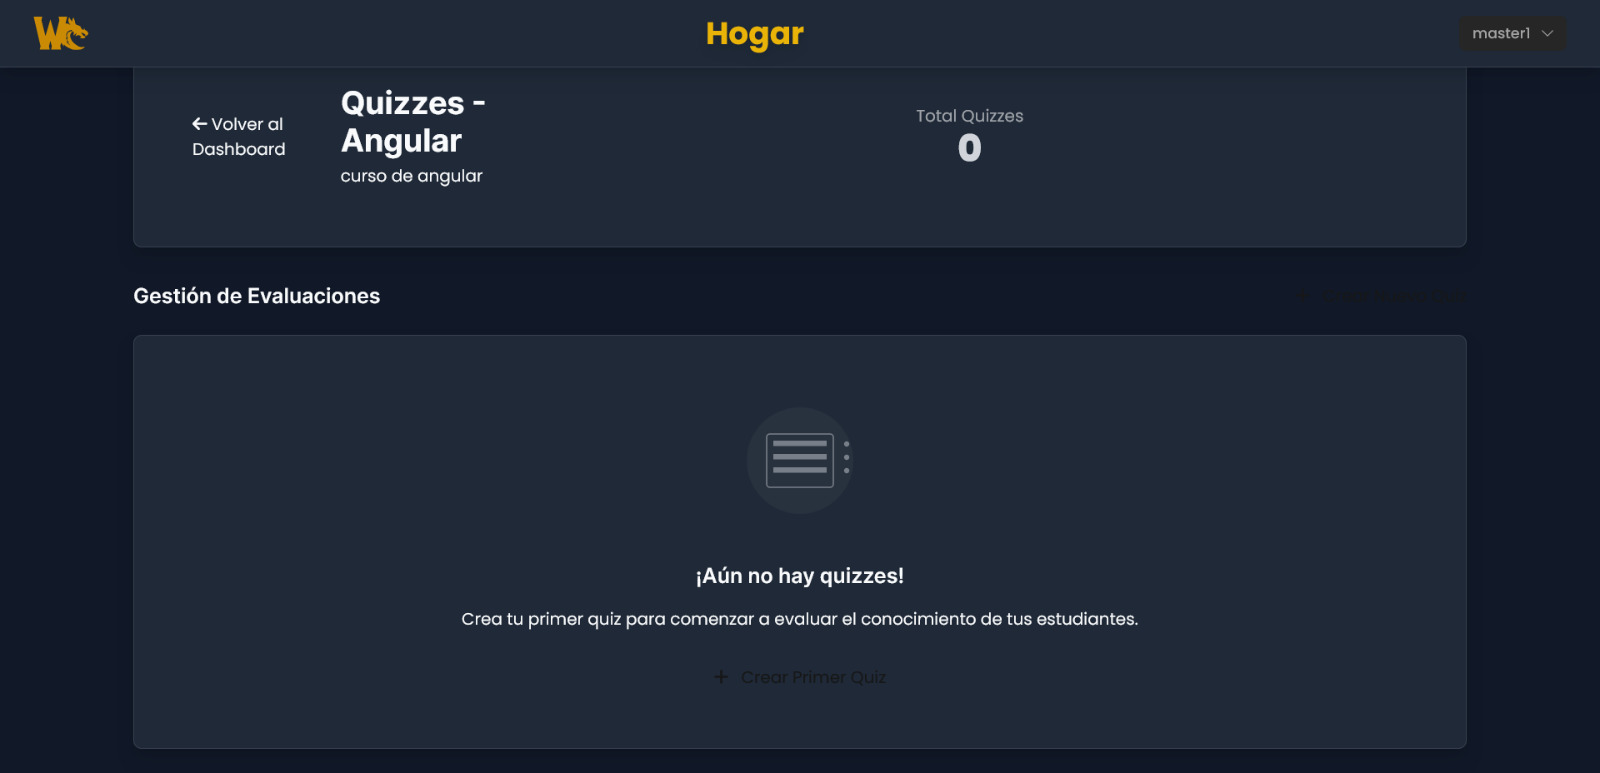
\includegraphics[width=0.75\textwidth]{images/pagina_web_gestion-de-evaluaciones.jpg}
	\caption{Sistema de evaluación y calificación de trabajos de estudiantes.}
	\label{fig:manual-evaluaciones}
\end{figure}

\paragraph{Analítica y seguimiento}

El sistema proporciona herramientas de analítica para monitorear el progreso:

\begin{itemize}
	\item \textbf{Panel de curso}: Métricas generales de participación y rendimiento
	\item \textbf{Gráficos de progreso}: Visualización temporal del avance del grupo
	\item \textbf{Análisis comparativo}: Identificación de misiones con mayor dificultad
	\item \textbf{Alertas tempranas}: Estudiantes en riesgo de abandono o bajo rendimiento
	\item \textbf{Reportes exportables}: Datos en formato CSV/PDF para análisis externo
\end{itemize}

\subsubsection{5.1.5 Manual para administradores}

\paragraph{Dashboard del administrador}

Los administradores institucionales tienen acceso a funcionalidades de gestión global:

\begin{itemize}
	\item \textbf{Gestión de usuarios}: Crear, editar y desactivar cuentas
	\item \textbf{Gestión de instituciones}: Configurar datos institucionales
	\item \textbf{Supervisión de cursos}: Vista global de todos los cursos activos
	\item \textbf{Reportes institucionales}: Métricas de uso y adopción
	\item \textbf{Configuración del sistema}: Parámetros globales de la plataforma
	\item \textbf{Auditoría}: Registro de actividades y eventos del sistema
\end{itemize}

\paragraph{Gestión de usuarios}

\textbf{Crear cuentas masivamente:}

\begin{enumerate}
	\item Ir a ``Administración'' > ``Usuarios'' > ``Importar''
	\item Descargar plantilla CSV
	\item Completar datos: email, nombre, rol, código institucional
	\item Subir archivo CSV
	\item Revisar y confirmar importación
	\item El sistema envía correos de activación automáticamente
\end{enumerate}

\textbf{Gestionar roles y permisos:}

\begin{itemize}
	\item \textbf{Superadministrador}: Control total del sistema
	\item \textbf{Administrador institucional}: Gestión de su institución
	\item \textbf{Coordinador académico}: Supervisión de departamentos
	\item \textbf{Docente}: Creación y gestión de cursos
	\item \textbf{Estudiante}: Participación en cursos
\end{itemize}

\paragraph{Configuración institucional}

\begin{enumerate}
	\item Acceder a ``Configuración'' > ``Institución''
	\item Configurar:
	\begin{itemize}
		\item Datos de la institución (nombre, logo, colores)
		\item Políticas de privacidad y términos de servicio
		\item Proveedores OAuth2 autorizados
		\item Dominios de correo institucional permitidos
		\item Integraciones con LMS (Canvas, Moodle)
		\item Configuración de Discord
	\end{itemize}
	\item Guardar cambios
\end{enumerate}

\paragraph{Monitoreo y reportes}

\begin{itemize}
	\item \textbf{Dashboard ejecutivo}: KPIs de adopción y uso
	\item \textbf{Reportes de engagement}: Tasas de participación por departamento
	\item \textbf{Análisis de rendimiento}: Métricas académicas agregadas
	\item \textbf{Auditoría de sistema}: Eventos de seguridad y accesos
	\item \textbf{Uso de recursos}: Consumo de almacenamiento y ancho de banda
\end{itemize}

\subsection{5.2 Manual del sistema}

El Manual del Sistema proporciona documentación técnica completa para el personal de TI encargado de instalar, configurar, mantener y resolver problemas de la plataforma. Incluye arquitectura del sistema, procedimientos de despliegue, configuración de servicios y guías de troubleshooting.

\subsubsection{5.2.1 Arquitectura del sistema}

\paragraph{Stack tecnológico}

\begin{table}[H]
	\centering
	\caption{Componentes tecnológicos del sistema.}
	\begin{tabular}{p{4cm} p{9cm}}
		\toprule
		Componente & Tecnología \\
		\midrule
		Frontend Web & Next.js 15.5.4, React 18, TypeScript 5 \\
		Entorno 3D & Three.js R150+, WebGL 2.0 \\
		Frontend Móvil & React Native (Expo) \\
		Backend API & Next.js API Routes (TypeScript) \\
		Base de Datos & PostgreSQL 15+ \\
		ORM & Prisma 5+ \\
		Autenticación & NextAuth.js con OAuth2 (Google, Microsoft) \\
		Almacenamiento & AWS S3 \\
		Notificaciones & Sistema de notificaciones integrado \\
		Analítica & Mixpanel / Google Analytics \\
		Contenedores & Docker 24+, Docker Compose \\
		Orquestación & Kubernetes 1.28+ (opcional) \\
		CI/CD & GitHub Actions, Vercel \\
		\bottomrule
	\end{tabular}
\end{table}

\paragraph{Diagrama de componentes}

El sistema se compone de los siguientes módulos principales:

\begin{itemize}
	\item \textbf{Cliente Web}: Aplicación Next.js con App Router que sirve la interfaz web y renderiza el entorno 3D con Three.js
	\item \textbf{Cliente Móvil}: Aplicación React Native (Expo) para Android e iOS
	\item \textbf{API Backend}: Next.js API Routes que implementan la lógica de negocio
	\item \textbf{Módulo de Autenticación}: NextAuth.js para OAuth2 y gestión de sesiones JWT
	\item \textbf{Base de Datos}: PostgreSQL con esquema gestionado por Prisma
	\item \textbf{Servicio de Almacenamiento}: AWS S3 para archivos y modelos 3D
	\item \textbf{Servicio de Notificaciones}: Sistema de notificaciones integrado en tiempo real
	\item \textbf{Integraciones Externas}: Conectores para Canvas LMS y Discord
\end{itemize}

\subsubsection{5.2.2 Requisitos del servidor}

\paragraph{Requisitos mínimos (100 usuarios concurrentes)}

\begin{table}[H]
	\centering
	\caption{Especificaciones mínimas del servidor.}
	\begin{tabular}{p{4cm} p{9cm}}
		\toprule
		Recurso & Especificación \\
		\midrule
		CPU & 4 cores (2.5 GHz) \\
		RAM & 8 GB \\
		Almacenamiento & 100 GB SSD \\
		Ancho de banda & 100 Mbps simétrico \\
		Base de Datos & PostgreSQL: 2 cores, 4 GB RAM, 50 GB SSD \\
		\bottomrule
	\end{tabular}
\end{table}

\paragraph{Requisitos recomendados (500+ usuarios concurrentes)}

\begin{table}[H]
	\centering
	\caption{Especificaciones recomendadas del servidor.}
	\begin{tabular}{p{4cm} p{9cm}}
		\toprule
		Recurso & Especificación \\
		\midrule
		CPU & 8+ cores (3.0 GHz) \\
		RAM & 16+ GB \\
		Almacenamiento & 500 GB SSD NVMe \\
		Ancho de banda & 1 Gbps simétrico \\
		Base de Datos & PostgreSQL: 4 cores, 16 GB RAM, 200 GB SSD \\
		Balanceador de Carga & Nginx o HAProxy \\
		\bottomrule
	\end{tabular}
\end{table}

\subsubsection{5.2.3 Instalación y despliegue}

\paragraph{Prerrequisitos}

\begin{itemize}
	\item Sistema operativo: Ubuntu 22.04 LTS o superior (recomendado)
	\item Node.js 18+ y npm 9+
	\item PostgreSQL 15+
	\item Docker 24+ y Docker Compose (opcional pero recomendado)
	\item Git para control de versiones
	\item Certificado SSL/TLS válido
\end{itemize}

\paragraph{Opción 1: Despliegue con Docker (Recomendado)}

\textbf{Paso 1: Clonar repositorio}

\begin{verbatim}
git clone https://github.com/institucion/warclass.git
cd warclass
\end{verbatim}

\textbf{Paso 2: Configurar variables de entorno}

Crear archivo \texttt{.env} en el directorio \texttt{web/}:

\begin{verbatim}
# Base de datos
DATABASE_URL="postgresql://user:password@db:5432/warclass"

# Autenticación
NEXTAUTH_URL="https://warclass.institucion.edu"
NEXTAUTH_SECRET="generate-random-secret-here"

# OAuth2 Providers
GOOGLE_CLIENT_ID="your-google-client-id"
GOOGLE_CLIENT_SECRET="your-google-client-secret"
MICROSOFT_CLIENT_ID="your-microsoft-client-id"
MICROSOFT_CLIENT_SECRET="your-microsoft-client-secret"

# Almacenamiento
S3_ENDPOINT="https://s3.amazonaws.com"
S3_BUCKET="warclass-storage"
S3_ACCESS_KEY="your-access-key"
S3_SECRET_KEY="your-secret-key"

# Integraciones
CANVAS_API_URL="https://canvas.institucion.edu/api/v1"
CANVAS_API_KEY="your-canvas-api-key"
DISCORD_BOT_TOKEN="your-discord-bot-token"
\end{verbatim}

\textbf{Paso 3: Copiar modelos 3D}

\begin{verbatim}
cd web
# Windows PowerShell
.\scripts\copy-models.ps1

# Linux/Mac
chmod +x scripts/copy-models.sh
./scripts/copy-models.sh
\end{verbatim}

\textbf{Paso 4: Construir y ejecutar contenedores}

\begin{verbatim}
docker-compose up -d
\end{verbatim}

\textbf{Paso 5: Ejecutar migraciones de base de datos}

\begin{verbatim}
docker-compose exec web npx prisma migrate deploy
docker-compose exec web npx prisma db seed
\end{verbatim}

\textbf{Paso 6: Verificar despliegue}

Acceder a \texttt{https://warclass.institucion.edu} para verificar que la aplicación esté funcionando.

\paragraph{Opción 2: Despliegue manual}

\textbf{Paso 1: Instalar dependencias del sistema}

\begin{verbatim}
# Ubuntu/Debian
sudo apt update
sudo apt install -y nodejs npm postgresql nginx

# Configurar PostgreSQL
sudo -u postgres createuser warclass -P
sudo -u postgres createdb warclass -O warclass
\end{verbatim}

\textbf{Paso 2: Clonar y configurar aplicación}

\begin{verbatim}
git clone https://github.com/institucion/warclass.git
cd warclass/web
npm install
\end{verbatim}

Configurar variables de entorno como en la opción Docker.

\textbf{Paso 3: Copiar modelos 3D}

\begin{verbatim}
chmod +x scripts/copy-models.sh
./scripts/copy-models.sh
\end{verbatim}

\textbf{Paso 4: Ejecutar migraciones}

\begin{verbatim}
npx prisma migrate deploy
npx prisma db seed
\end{verbatim}

\textbf{Paso 5: Construir aplicación}

\begin{verbatim}
npm run build
\end{verbatim}

\textbf{Paso 6: Configurar servicio systemd}

Crear \texttt{/etc/systemd/system/warclass.service}:

\begin{verbatim}
[Unit]
Description=Warclass Application
After=network.target postgresql.service

[Service]
Type=simple
User=warclass
WorkingDirectory=/opt/warclass/web
Environment=NODE_ENV=production
ExecStart=/usr/bin/npm start
Restart=always

[Install]
WantedBy=multi-user.target
\end{verbatim}

Activar servicio:

\begin{verbatim}
sudo systemctl enable warclass
sudo systemctl start warclass
\end{verbatim}

\textbf{Paso 7: Configurar Nginx como reverse proxy}

Crear \texttt{/etc/nginx/sites-available/warclass}:

\begin{verbatim}
server {
    listen 80;
    server_name warclass.institucion.edu;
    return 301 https://$server_name$request_uri;
}

server {
    listen 443 ssl http2;
    server_name warclass.institucion.edu;

    ssl_certificate /etc/letsencrypt/live/warclass.institucion.edu/fullchain.pem;
    ssl_certificate_key /etc/letsencrypt/live/warclass.institucion.edu/privkey.pem;

    location / {
        proxy_pass http://localhost:3000;
        proxy_http_version 1.1;
        proxy_set_header Upgrade $http_upgrade;
        proxy_set_header Connection 'upgrade';
        proxy_set_header Host $host;
        proxy_cache_bypass $http_upgrade;
        proxy_set_header X-Real-IP $remote_addr;
        proxy_set_header X-Forwarded-For $proxy_add_x_forwarded_for;
        proxy_set_header X-Forwarded-Proto $scheme;
    }
}
\end{verbatim}

Activar configuración:

\begin{verbatim}
sudo ln -s /etc/nginx/sites-available/warclass /etc/nginx/sites-enabled/
sudo nginx -t
sudo systemctl reload nginx
\end{verbatim}

\subsubsection{5.2.4 Configuración del sistema}

\paragraph{Configuración de base de datos}

\textbf{Optimizaciones de PostgreSQL:}

Editar \texttt{/etc/postgresql/15/main/postgresql.conf}:

\begin{verbatim}
# Conexiones
max_connections = 200

# Memoria
shared_buffers = 4GB
effective_cache_size = 12GB
maintenance_work_mem = 1GB
work_mem = 16MB

# WAL
wal_buffers = 16MB
checkpoint_completion_target = 0.9

# Consultas
random_page_cost = 1.1
effective_io_concurrency = 200
\end{verbatim}

\textbf{Índices recomendados:}

\begin{verbatim}
-- Usuarios
CREATE INDEX idx_users_email ON users(email);
CREATE INDEX idx_users_role ON users(role);

-- Misiones
CREATE INDEX idx_missions_course_id ON missions(course_id);
CREATE INDEX idx_missions_status ON missions(status);
CREATE INDEX idx_missions_deadline ON missions(deadline);

-- Entregas
CREATE INDEX idx_submissions_mission_id ON submissions(mission_id);
CREATE INDEX idx_submissions_student_id ON submissions(student_id);
CREATE INDEX idx_submissions_status ON submissions(status);

-- Progreso
CREATE INDEX idx_progress_student_id ON progress(student_id);
CREATE INDEX idx_progress_course_id ON progress(course_id);
\end{verbatim}

\paragraph{Configuración de almacenamiento S3}

\textbf{Configurar bucket en AWS S3:}

\begin{enumerate}
	\item Acceder a la consola de AWS S3
	\item Crear un nuevo bucket llamado \texttt{warclass-storage}
	\item Configurar políticas de acceso y CORS
	\item Generar credenciales de acceso (Access Key y Secret Key)
	\item Configurar las credenciales en el archivo \texttt{.env}
\end{enumerate}

\subsubsection{5.2.5 Mantenimiento y operaciones}

\paragraph{Backups automatizados}

\textbf{Script de backup de PostgreSQL:}

Crear \texttt{/opt/scripts/backup-postgres.sh}:

\begin{verbatim}
#!/bin/bash
BACKUP_DIR="/backups/postgres"
TIMESTAMP=$(date +"%Y%m%d_%H%M%S")
mkdir -p $BACKUP_DIR

pg_dump -U warclass -d warclass | gzip > \
  $BACKUP_DIR/warclass_$TIMESTAMP.sql.gz

# Retener últimos 7 días
find $BACKUP_DIR -name "*.sql.gz" -mtime +7 -delete
\end{verbatim}

\textbf{Configurar cron:}

\begin{verbatim}
# Backup diario a las 2 AM
0 2 * * * /opt/scripts/backup-postgres.sh
\end{verbatim}

\paragraph{Monitoreo del sistema}

\textbf{Métricas clave a monitorear:}

\begin{itemize}
	\item \textbf{Aplicación}: Tiempo de respuesta, tasa de errores, uso de CPU/RAM
	\item \textbf{Base de datos}: Conexiones activas, queries lentas, tamaño de BD
	\item \textbf{Almacenamiento}: Espacio disponible en AWS S3, IOPS
	\item \textbf{Red}: Ancho de banda, latencia, conexiones concurrentes
\end{itemize}

\textbf{Herramientas recomendadas:}

\begin{itemize}
	\item Prometheus + Grafana para métricas
	\item Sentry para tracking de errores
	\item pgAdmin para administración de PostgreSQL
	\item AWS CloudWatch para monitoreo de S3
	\item Nginx Amplify para monitoreo de Nginx
\end{itemize}

\paragraph{Actualizaciones del sistema}

\textbf{Proceso de actualización:}

\begin{enumerate}
	\item Notificar a usuarios sobre ventana de mantenimiento
	\item Realizar backup completo
	\item Descargar nueva versión:
\begin{verbatim}
git fetch origin
git checkout v2.0.0  # versión específica
\end{verbatim}
	\item Instalar nuevas dependencias:
\begin{verbatim}
npm install
\end{verbatim}
	\item Ejecutar migraciones:
\begin{verbatim}
npx prisma migrate deploy
\end{verbatim}
	\item Reconstruir aplicación:
\begin{verbatim}
npm run build
\end{verbatim}
	\item Reiniciar servicios:
\begin{verbatim}
sudo systemctl restart warclass
# o con Docker:
docker-compose down && docker-compose up -d
\end{verbatim}
	\item Verificar funcionamiento y logs
	\item Si hay problemas, revertir al backup
\end{enumerate}

\subsubsection{5.2.6 Resolución de problemas}

\paragraph{Problemas comunes y soluciones}

\textbf{Problema: Modelos 3D no cargan (Error 404)}

\textit{Causa:} Los modelos no fueron copiados a \texttt{public/}

\textit{Solución:}
\begin{verbatim}
cd web
./scripts/copy-models.sh  # Linux/Mac
.\scripts\copy-models.ps1  # Windows
npm run build
\end{verbatim}

\textbf{Problema: Error de conexión a base de datos}

\textit{Causa:} PostgreSQL no está corriendo o credenciales incorrectas

\textit{Solución:}
\begin{verbatim}
# Verificar servicio
sudo systemctl status postgresql

# Verificar conexión
psql -U warclass -d warclass -h localhost

# Revisar variable DATABASE_URL en .env
\end{verbatim}

\textbf{Problema: Sesiones de usuarios expiran rápidamente}

\textit{Causa:} Configuración incorrecta de NextAuth.js o tokens JWT

\textit{Solución:}
\begin{verbatim}
# Verificar variable NEXTAUTH_SECRET en .env
# Revisar configuración de expiración de tokens
# Revisar logs de la aplicación
docker-compose logs web
\end{verbatim}

\textbf{Problema: Rendimiento lento del entorno 3D}

\textit{Causa:} GPU del cliente no compatible con WebGL 2.0 o modelos no optimizados

\textit{Solución:}
\begin{itemize}
	\item Verificar compatibilidad WebGL del navegador: \texttt{https://get.webgl.org/webgl2/}
	\item Optimizar modelos 3D (reducir polígonos, comprimir texturas)
	\item Habilitar hardware acceleration en el navegador
	\item Actualizar drivers de GPU
\end{itemize}

\textbf{Problema: Notificaciones no funcionan}

\textit{Causa:} Sistema de notificaciones mal configurado o permisos del navegador

\textit{Solución:}
\begin{itemize}
	\item Verificar que el usuario haya otorgado permisos de notificaciones
	\item Comprobar que el sistema de notificaciones esté activo
	\item Revisar logs del navegador para errores
	\item Verificar conectividad de WebSocket si se usa comunicación en tiempo real
\end{itemize}

\paragraph{Logs del sistema}

\textbf{Ubicación de logs:}

\begin{itemize}
	\item Aplicación: \texttt{/var/log/warclass/app.log}
	\item PostgreSQL: \texttt{/var/log/postgresql/postgresql-15-main.log}
	\item Nginx: \texttt{/var/log/nginx/access.log} y \texttt{/var/log/nginx/error.log}
\end{itemize}

\textbf{Comandos útiles para revisar logs:}

\begin{verbatim}
# Ver logs en tiempo real
tail -f /var/log/warclass/app.log

# Buscar errores recientes
grep -i error /var/log/warclass/app.log | tail -50

# Logs con Docker
docker-compose logs -f web
docker-compose logs --tail=100 web
\end{verbatim}

\subsubsection{5.2.7 Seguridad}

\paragraph{Mejores prácticas de seguridad}

\begin{itemize}
	\item \textbf{HTTPS obligatorio}: Forzar HTTPS para todas las conexiones
	\item \textbf{Firewall}: Configurar firewall para permitir solo puertos necesarios (80, 443)
	\item \textbf{Actualizaciones}: Mantener sistema operativo y dependencias actualizadas
	\item \textbf{Contraseñas}: Usar contraseñas fuertes y únicas para servicios
	\item \textbf{Backups}: Almacenar backups en ubicación separada y encriptada
	\item \textbf{Auditoría}: Revisar logs regularmente en busca de actividad sospechosa
	\item \textbf{Rate limiting}: Configurar límites de solicitudes para prevenir abuso
	\item \textbf{CORS}: Configurar CORS apropiadamente en API routes
	\item \textbf{CSP}: Implementar Content Security Policy headers
	\item \textbf{Sanitización}: Validar y sanitizar todas las entradas de usuario
\end{itemize}

\paragraph{Configuración de firewall}

\begin{verbatim}
# UFW (Ubuntu)
sudo ufw default deny incoming
sudo ufw default allow outgoing
sudo ufw allow ssh
sudo ufw allow http
sudo ufw allow https
sudo ufw enable
\end{verbatim}

\paragraph{Certificados SSL/TLS}

\textbf{Generar certificado con Let's Encrypt:}

\begin{verbatim}
sudo apt install certbot python3-certbot-nginx
sudo certbot --nginx -d warclass.institucion.edu
sudo certbot renew --dry-run
\end{verbatim}

\subsubsection{5.2.8 Escalabilidad}

\paragraph{Escalamiento horizontal}

Para manejar mayor carga de usuarios, se puede escalar horizontalmente:

\begin{enumerate}
	\item \textbf{Load Balancer}: Configurar balanceador de carga (Nginx, HAProxy)
	\item \textbf{Múltiples instancias}: Desplegar múltiples contenedores de la aplicación
	\item \textbf{Base de datos replicada}: Configurar réplicas de lectura de PostgreSQL
	\item \textbf{CDN}: Usar AWS CloudFront para servir assets estáticos y modelos 3D
	\item \textbf{Auto-scaling}: Configurar auto-scaling en AWS para ajustar recursos según demanda
\end{enumerate}

\paragraph{Configuración con Kubernetes}

Para entornos de producción grandes, se recomienda Kubernetes:

\begin{verbatim}
# Desplegar con Helm
helm repo add warclass https://charts.warclass.io
helm install warclass warclass/warclass \
  --set database.host=postgres.example.com \
  --set s3.bucket=warclass-storage \
  --set replicas=3
\end{verbatim}

El sistema se autoescalará según carga de CPU/memoria configurada en HPA (Horizontal Pod Autoscaler).

\section{CONCLUSIONES}

\textit{Por desarrollar}

\section{RECOMENDACIONES}

\textit{Por desarrollar}

\renewcommand\refname{\large\textbf{Referencias}}
\bibliography{bib/references}

\end{document}
